\documentclass[10pt,journal,compsoc]{IEEEtran}

% *** CITATION PACKAGES ***
%
\ifCLASSOPTIONcompsoc
  \usepackage[nocompress]{cite}
\else
  % normal IEEE
  \usepackage{cite}
\fi

\usepackage{float}
% *** GRAPHICS RELATED PACKAGES ***
%

\ifCLASSINFOpdf
  \usepackage[pdftex]{graphicx}
  %declare the path(s) where your graphic files are
  \graphicspath{{../pdf/}{../jpeg/}}
  % and their extensions so you won't have to specify these with
  % every instance of \includegraphics
 \DeclareGraphicsExtensions{.pdf,.jpeg,.png}
\else
  % or other class option (dvipsone, dvipdf, if not using dvips). graphicx
  % will default to the driver specified in the system graphics.cfg if no
  % driver is specified.
    \usepackage[dvips]{graphicx}
  % declare the path(s) where your graphic files are
    \graphicspath{{../eps/}}
  % and their extensions so you won't have to specify these with
  % every instance of \includegraphics
    \DeclareGraphicsExtensions{.eps}
\fi

\newcommand\MYhyperrefoptions{bookmarks=true,bookmarksnumbered=true,
pdfpagemode={UseOutlines},plainpages=false,pdfpagelabels=true,
colorlinks=true,linkcolor={black},citecolor={black},urlcolor={black}}

\hyphenation{op-tical net-works semi-conduc-tor}


\begin{document}

\title{Concurrency and Parallelism}

\author{Miguel~Anci\~aes -~\IEEEmembership{~43367}, Ricardo~Amaral -~\IEEEmembership{~43368}, Tiago~Sousa -~\IEEEmembership{~43364}% <-this % stops a space
}

\IEEEtitleabstractindextext{%
\begin{abstract}

1. The problem was to convert patterns from their Serial version to Parallel version\\
2. This is interesting so we can find a way to optimize a program to be more efficient\\
3. Our approach was to divide the work between workers in most patterns to overcome some heavy tasks that would take if it was done in serial. \\
4. After several Tests and based on or results we've learned that Paralyzing is not always the best solution for all patterns and depends on the input given. But in general for bigger problems with some hard work per iteration, parallelize is a great solution for many patterns.
\end{abstract}

}
% make the title area
    

\IEEEdisplaynontitleabstractindextext

\IEEEpeerreviewmaketitle

\maketitle

\section{Introduction}
In this Project it was proposed to implement a Parallel version of several working patterns in which the challenge was to optimize the code to be as fast and as scalable as possible , in particular, Map, Reduce, Scan, Pack, Gather, Scatter, Pipeline and Farm. Due to the introduction and further development of Cilk + in the lab's, the parallelization was implemented with it. The use of the Cilk + was restricted, the challenge was that the reducers available in the Cilk library, were not allowed to use.
    
The challenge was not only to parallelize the code but to be aware of its optimization , specifically, for the given arguments and inputs, was compensated enough to parallelize, or given the same input the sequential version was good enough, or better than its parallelization. 
    
So for better understanding of its complexity and implementation a research had to be done and considered for each individual pattern. After an intense and considered research, and some reflection between all the members of the group, we implemented what we think, was the best approach for each pattern with the different inputs given. 
    
The development of each individual pattern was done in group. We think with this approach, gave us a wider view of the problem, and  have  more counter arguments, to achieve a better solution for the specific problem.
    
    



\section{Architecture / Model / Solution}
For the  Map pattern, a function is applied to all elements of a collection, usually producing a new collection with the same shape as the input.

For the Reduce pattern, it combines every element in a collection into a single element using an associative combiner function.

For the Scan pattern it computes all partial reductions of a collection. In other words, for every output position, a reduction of the input up to that point is computed. 

For the Pack pattern it can be used to eliminate unused space in a collection.It takes as input a collection and a Boolean condition (or flag) for each element of that collection. It discards the elements of the input collection for which the condition is false and then packs together the surviving elements into a dense output collection, eliminating the gaps. 

For the Gather pattern it reads a collection of data from another data collection, given a collection of indices.

For the Scatter pattern is the inverse of the gather pattern: A set of input data and a set of indices is given, but each element of the input is written at the given location, not read.

For the Pipeline pattern it connects tasks in a producer consumer relationship. Conceptually, all stages of the pipeline are active at once, and each stage can maintain state that can be updated as data flows through them.

For the Farm pattern it computes in parallel a function F over all the items appearing in the input stream, therefore, an item of f is generated in the output of each item, of the input stream. The computations performed by f for the items in the stream, are completely independent to each other, so they can be processed in parallel.


%Describe your approach/solution in a way that is as independent
%as possible form your implementation. What you describe here should be (as much
%as possible) neutral to the programmin language and to the parallelization framework being
%used.

\section{Implementation}

\subsection{Map}

For the Map Pattern, our approach was to make use of Cilk for to apply the same operation to all values, since that there are no dependencies between data, we are looking at a truly embarrassingly parallel computation where there is no need for interactions between separate processes.

\subsection{Reduce}

Unlike the map pattern, the reduce pattern does have dependencies between data, since we need the computation from other processes has an input. We decided to paralyze the problem into multiple phases where in each phase computations are performed in parallel two by two across the data array and the results are written in specific positions. Then, we repeat the process for making the computations two by two, but for the output arrays of the previous iteration until only on result exists. In our solution, workers are given a position \textbf{i} and \textbf{i + gap}, where i is never shared between processes and gap starts at 1, and applies the worker's function between the two data positions and stores them in position \textbf{i}. 

Then we double the value of the \textbf{gap} variable in the purpose of applying the same thinking as before but for the only for the results of the previous iterations.

We then continue with the next ones until we have a \textbf{gap} between results bigger than the size of the input array. That means we have reached the reduced value.

\subsection{Scan}

For the Scan Pattern, we implemented with the concept of a specific lecture given in the classes, specifically lecture ten, where we make use of The Prefix (Scan) Sum Problem, where the parallel-prefix algorithm does two passes, the first pass builds a tree bottom-up, and the seconds pass traverses the tree top-down, in which we nominated on our code by upsweep, and downsweep.
To achieve this result we've implemented two solutions, one where we use an actual tree structure where we need to fully build the tree so then we can downsweep it, and other solution that only needs one auxiliary array to store the upsweep result so on the downsweep we could get all values with auxiliary array in combination with source array.

We've kept the second solution because it's structure is much lighter then the tree structure solution.

\subsection{Pack}

For the Pack Pattern, we used took the filter array and passed it through the scan pattern implemented earlier. Since the map function needs a worker, we implemented a special worker that sums variables of \textbf{int} type. That way we have an auxiliary array to, in parallel, know how to eliminate the unwanted elements of the data array. Since the filter is a bitmap, an array of zeros and ones, the scan of that array will result in an array where there are only increases of one. We used a \textbf{cilk for} to evaluate the result of the scan for an increase and kept the input values corresponding to that increase. 

\subsection{Gather}

For the Gather Pattern, we decided to use only a Cilk for due to its independence, and to test several experiments with the nFilter to take our conclusions.

\subsection{Scatter}

For the Scatter Pattern, we implemented two types of solutions, deterministic and non-deterministic. The non-deterministic solution is the simplest and we just need to parallelize the for cycle and ignore the cases where two or more positions of filter array has the same index. This results in a conflict on the output array. On the other hand, for the deterministic solution, conflicts can't be ignored. So for the non-deterministic solution we need an extra step to see if there's a conflict and resolve it in several ways. Inside the non-deterministic solution we've implemented three approach's, make the least amount override the greater amount, make the greater amount override the least amount and, as last solution, keep always the first setted value on the output array. In terms of performance, and final decision, we've kept the non-deterministic solution since it performs slightly better. 

\subsection{Pipeline}

To implement the pipeline pattern we assume that each worker function of the worker input list has the id equal to its position on that array. We also keep an auxiliary array with size equals to the input's size, where each position relates to the corresponding data item, and the value stored in that position corresponds to the next worker id on which this item is going to be processed. The auxiliary array in initialized with all values equals to zero. That means that the next worker that is going to process all data items is set to the worker 0.

With this architecture when can keep track of which data item is currently being processed by each worker. 

When a data item leaves a worker (it is processed and written to the output), it increments the auxiliary array value on the position corresponding to the current data item, indicating to that worker to process another piece of data and to the next worker that this current data it's ready to be processed again by the next function. Data items follow the path of the workers correctly, and all workers are busy until all the input is processed.

Workers only stop processing data when there is no more data to process.

\subsection{Farm}

For the Farms Pattern, our approach was to use every worker available to loop until there were no more elements in the queue. This queue is created on function start and has all elements from the array source. In this solution we have to be careful with conflicts on pop's from the queue. To prevent this from happening we've used a lock system, where where we lock the queue, pop an element and then unlock the queue for other threads to use. With this solution is a significantly time gain if the time it takes to do the work on each element is greater than the time it takes to lock, pop and unlock an element.

\section{Experimental evaluation}
% How did you make your functional/correctness and performance
%evaluation? Were there are relevant results? How do you explain them?

For our experiments, due to the heavy Load of tasks, and experiments on the College Computer we concluded that the results shown when testing were having a huge impact on the final results, so our experiments were tested with an average of at least of ten attempts to get a more accurate results, and to be certain of the output, we tested our experiments in our computer with a consider quad-core Processor, with at least 8gb of ram. 

\begin{figure}[!htb]
\hspace*{-0.24in}
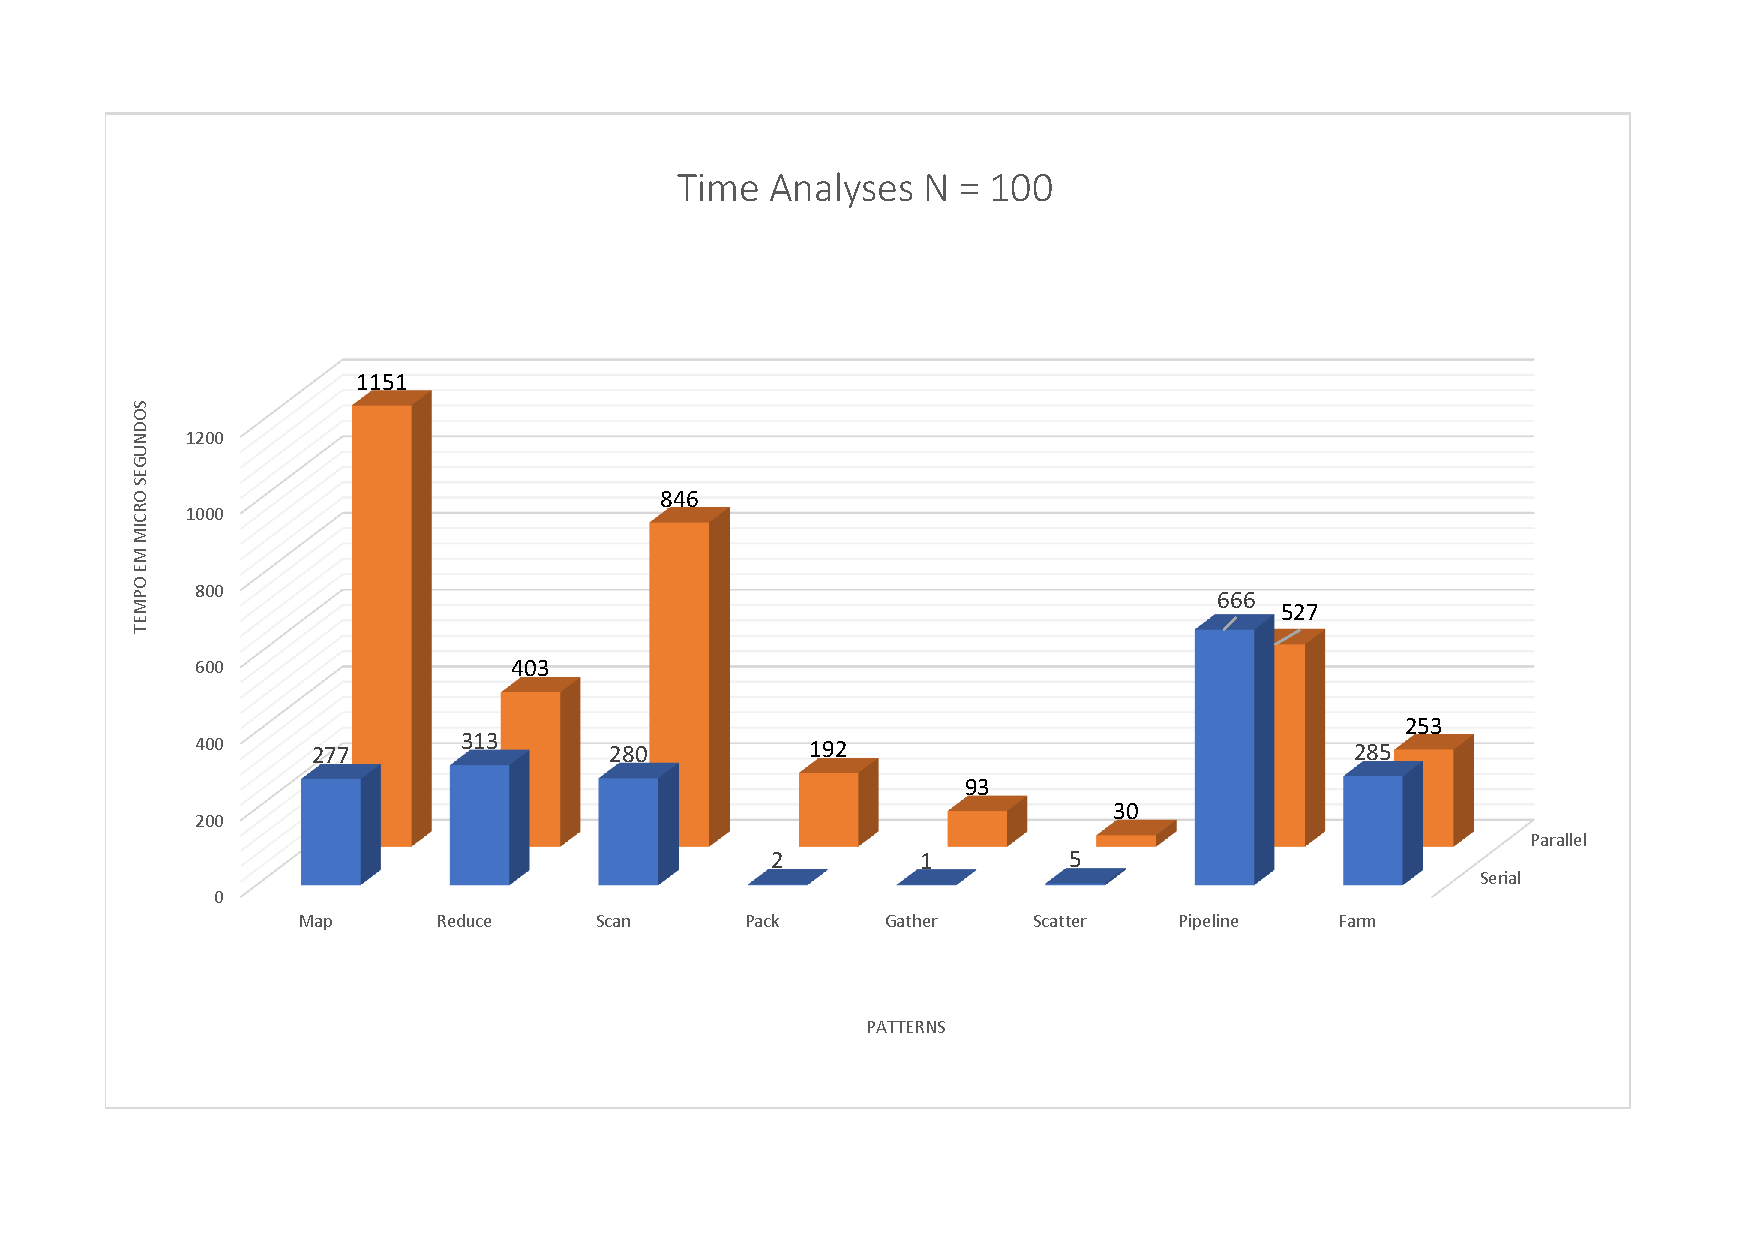
\includegraphics[ height=6cm,width=9.44cm]{jpeg/n=100.pdf}
\caption{N=100}
\label{figura:n100}
\end{figure}

For N=100 represented in (Fig. 1.) we conclude that for such a small problem only Pipeline pattern is slightly more fast if we parallelize, otherwise serial wins or ties with parallel version for all other patterns.
The two biggest gaps are visible on Map pattern and Scan pattern.

\begin{figure}[H]
\hspace*{-0.24in}
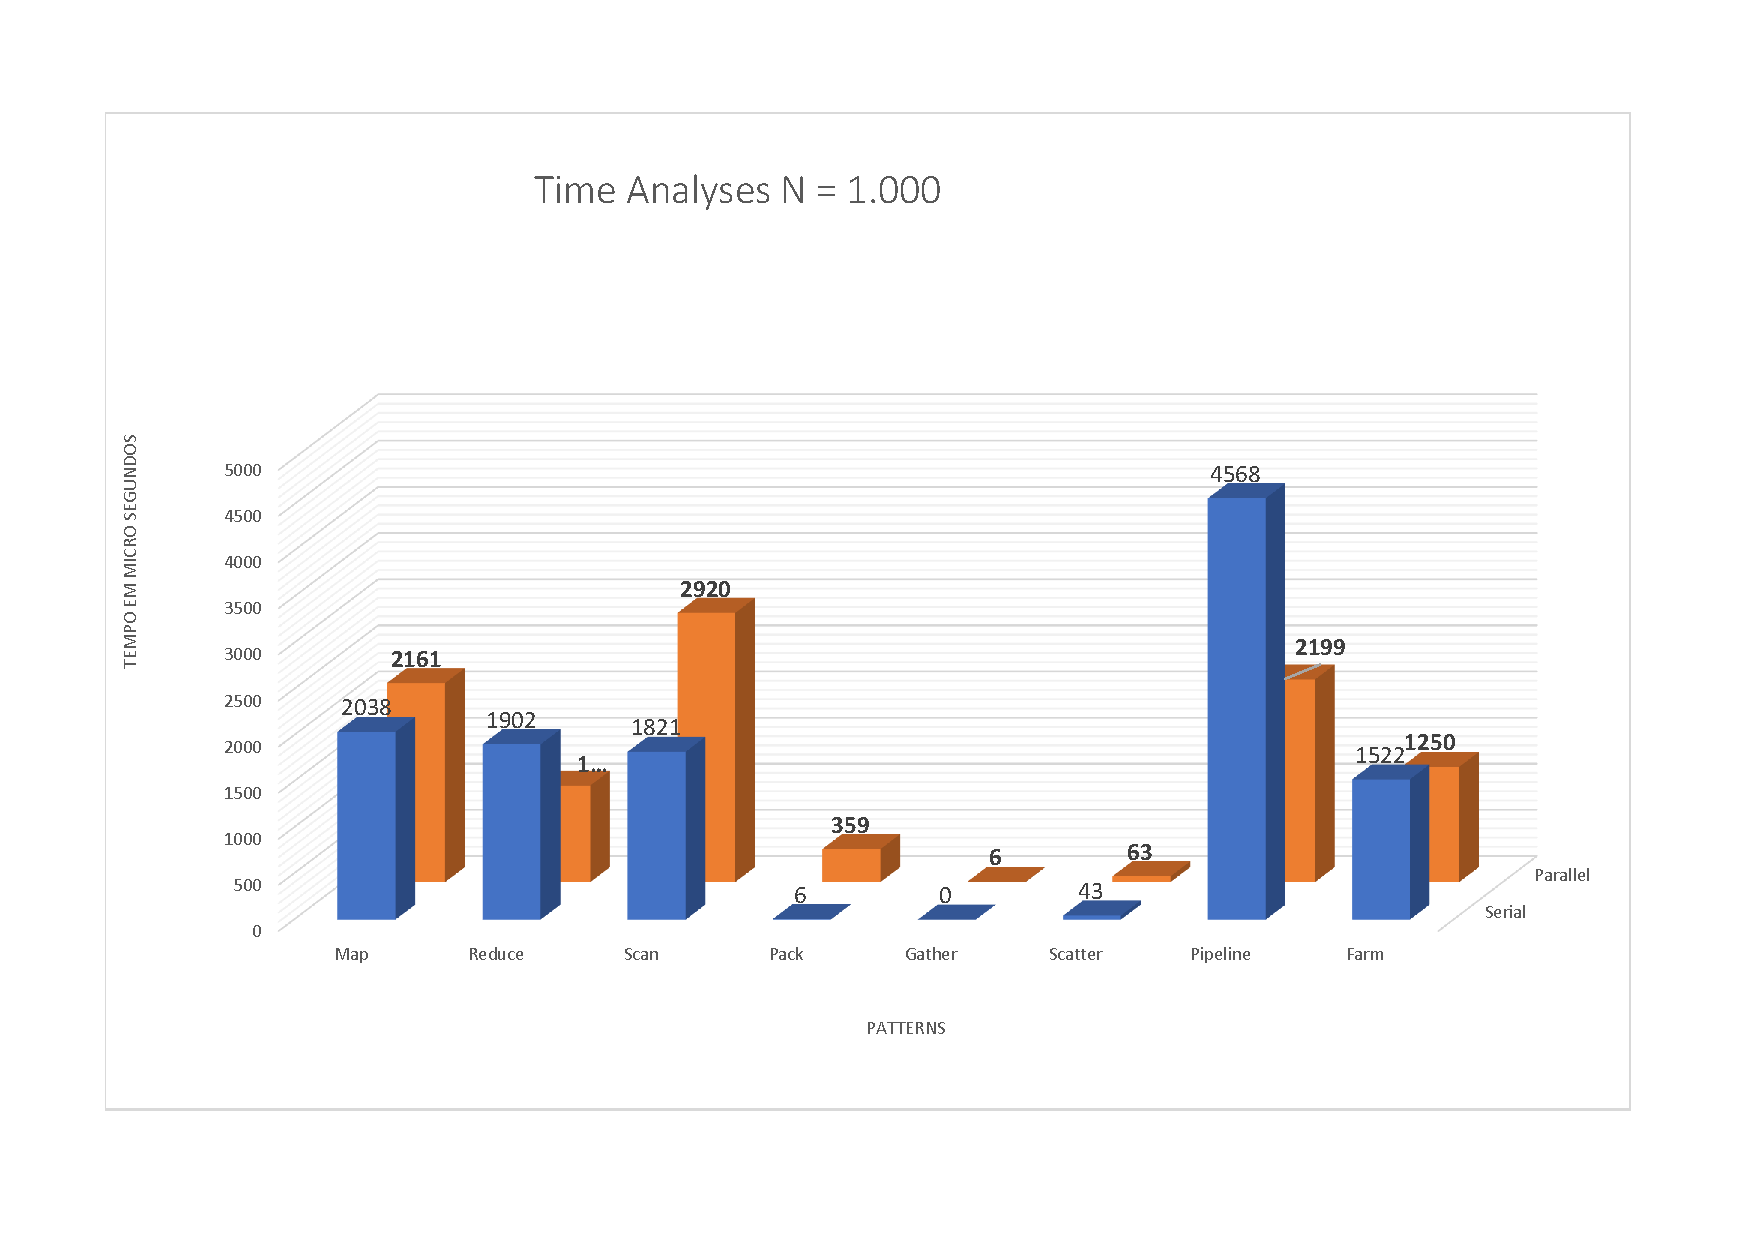
\includegraphics[height=6cm,width=9.44cm]{jpeg/n=1000.pdf}
\caption{N=1.000}
\label{figura:n1000}
\end{figure}

For N=1.000 represented in (Fig.2), the main conclusion we can get from the results is a huge deficit in the Pipeline pattern in compare with the previous graph (Fig. 1.). Also important to notice a much higher balance between serial and parallel times. With parallel even doing better on the Reduce patter.

\begin{figure}[H]
\hspace*{-0.24in}
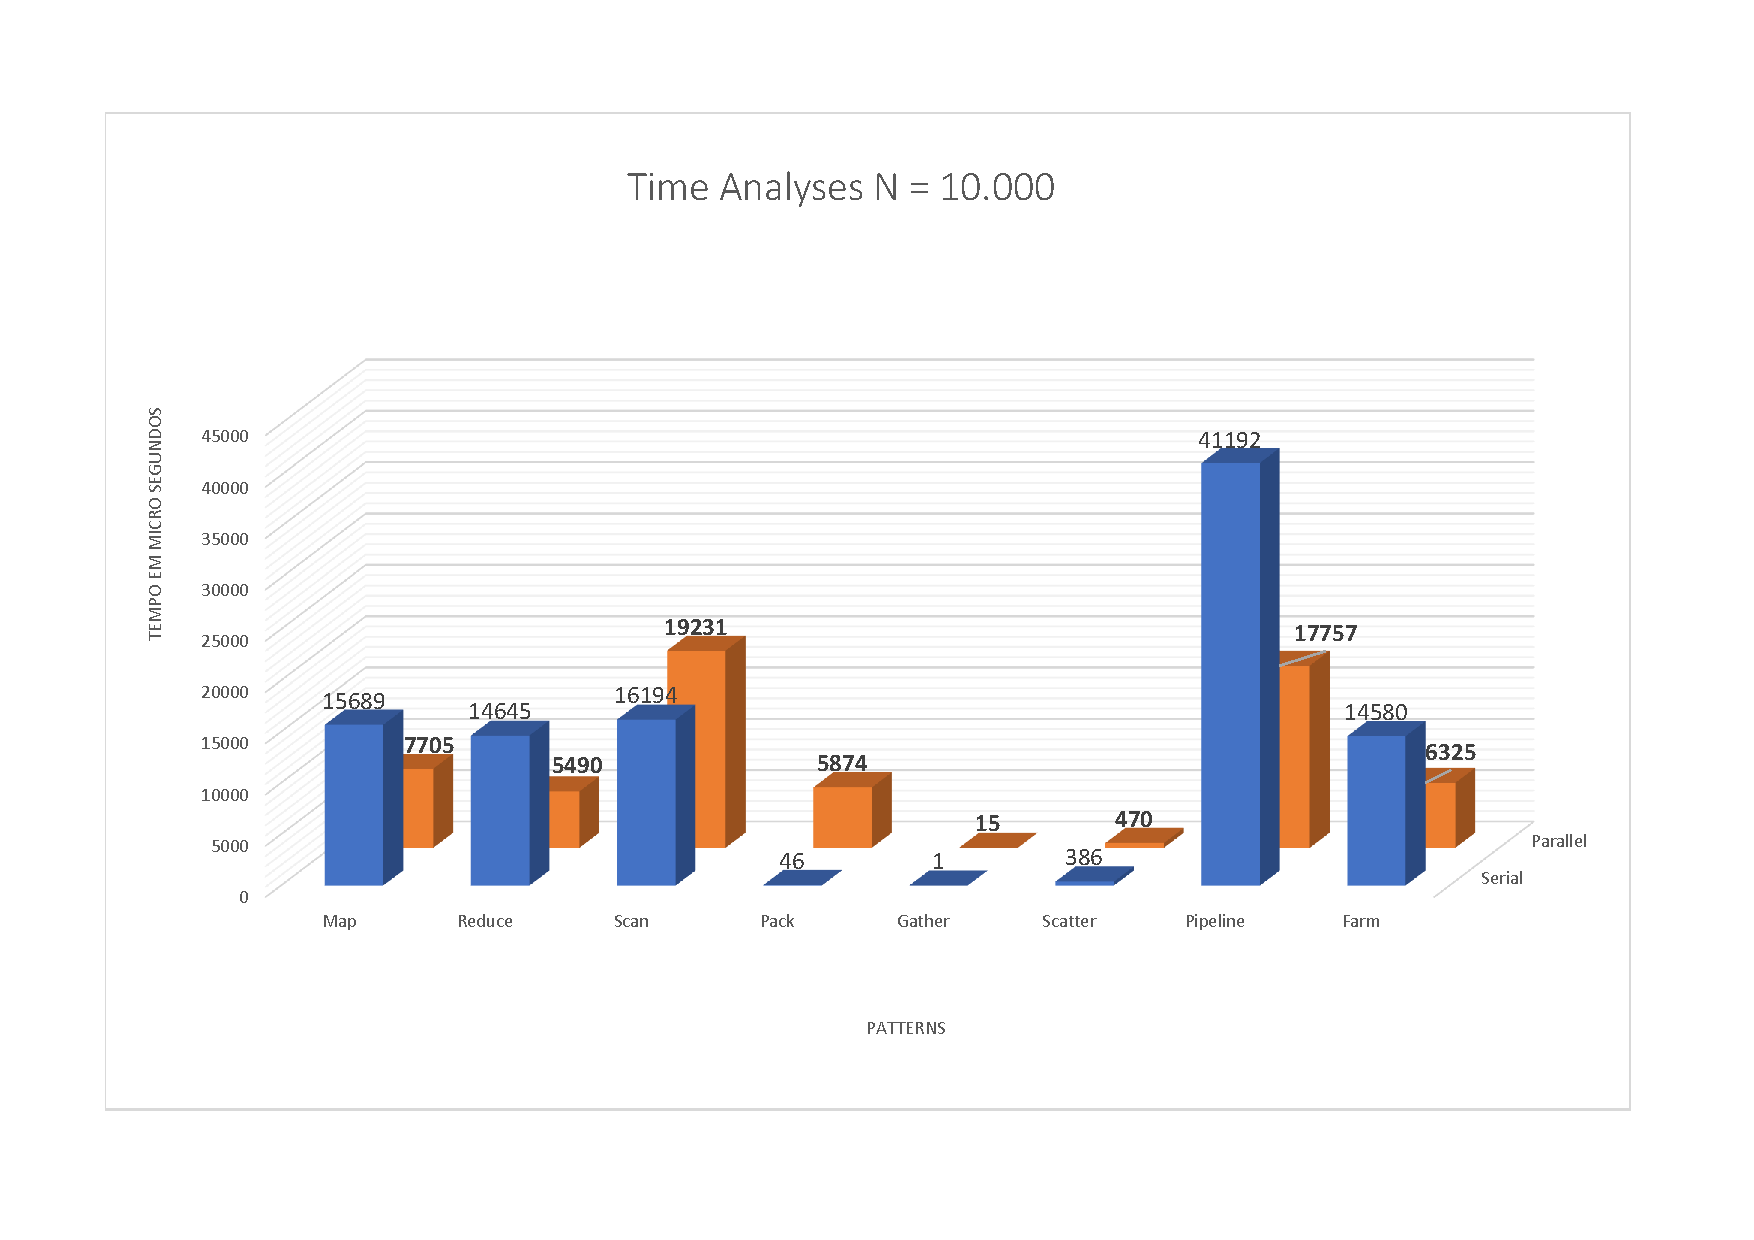
\includegraphics[height=6cm,width=9.44cm]{jpeg/n=10000.pdf}
\caption{N=10.000}
\label{figura:n10000}
\end{figure}

For N=10.000 represented in (Fig. 3.) we reach a point where parallel is behind serial only in two patterns, Scan pattern and Pack pattern. With parallel times on other patterns still decreasing when compare with serial times.

\begin{figure}[H]
\hspace*{-0.24in}
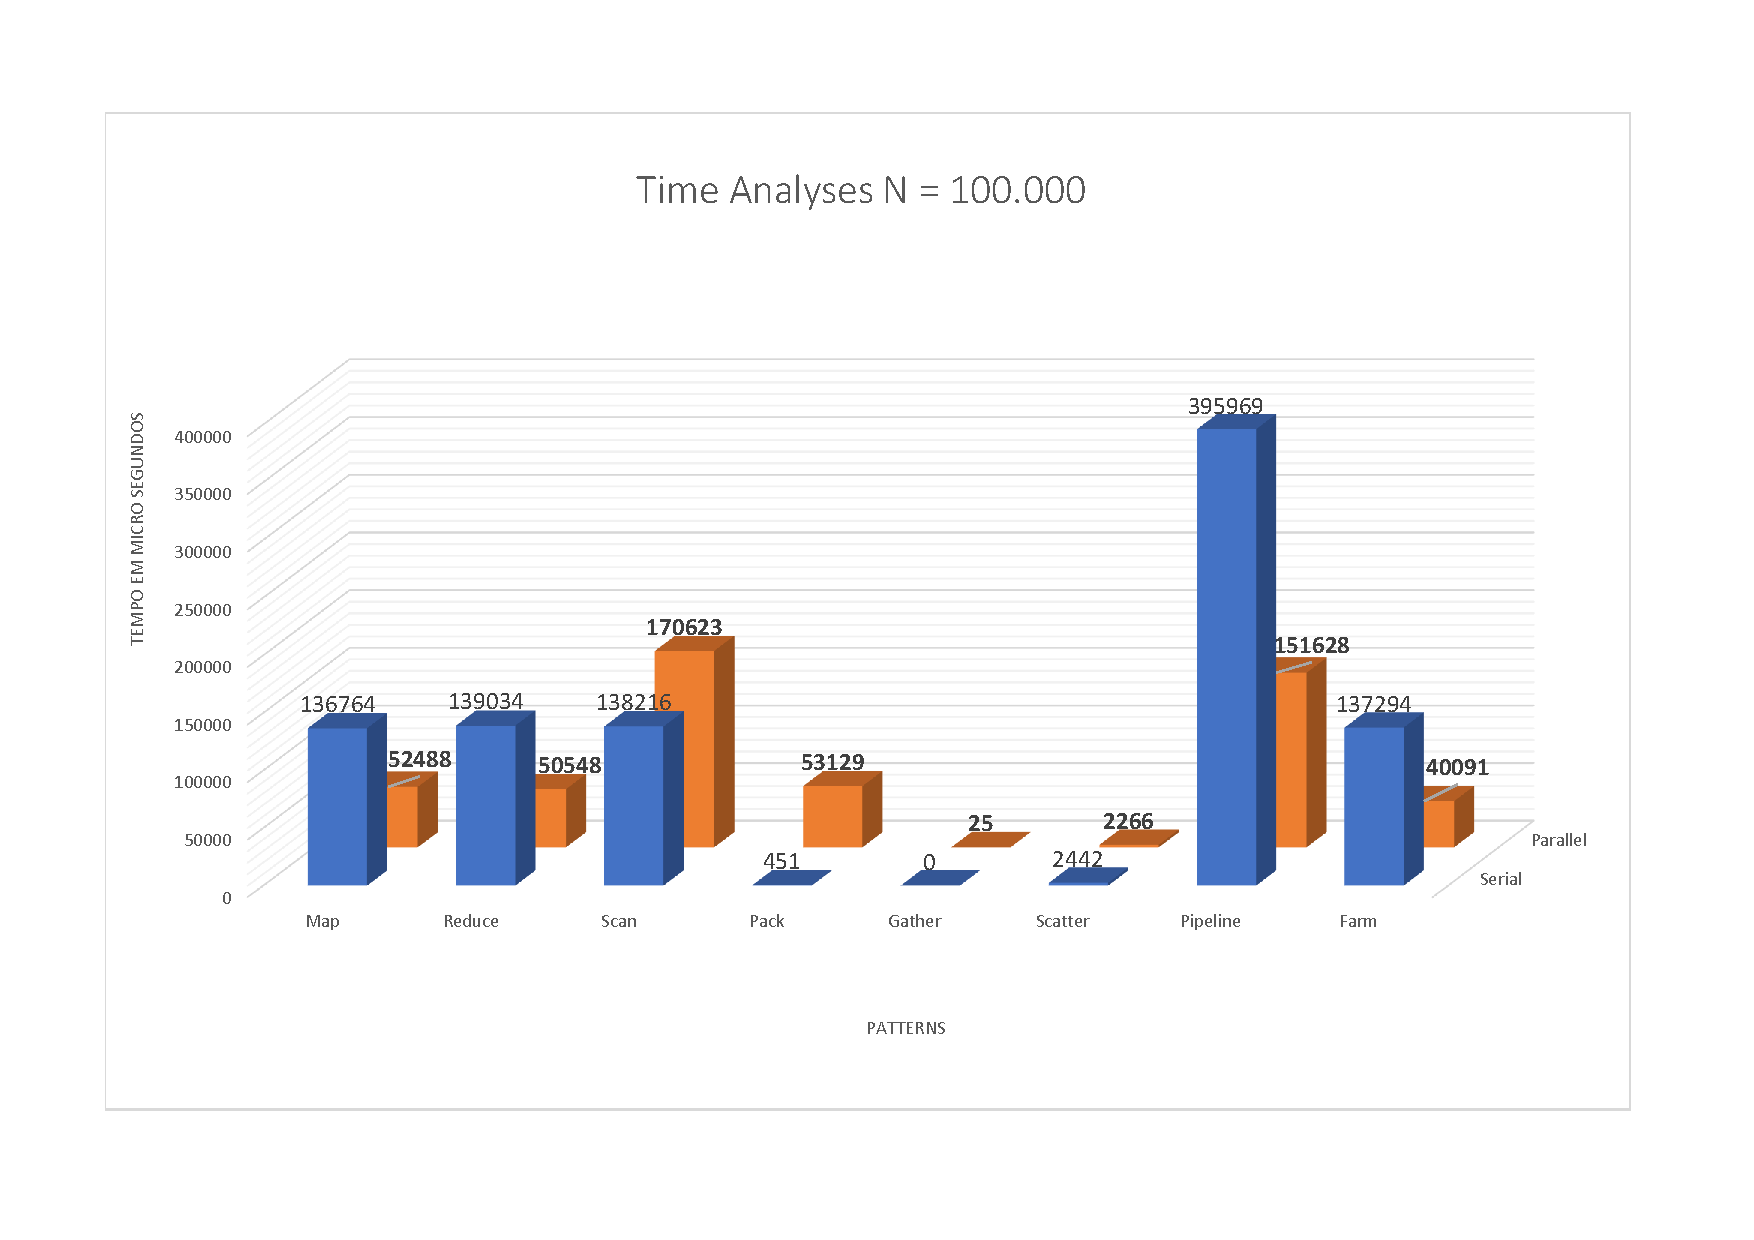
\includegraphics[height=6cm,width=9.44cm]{jpeg/n=100000.pdf}
\caption{N=100.000}
\label{figura:n100000}
\end{figure}

For N=100.000 represented in (Fig. 3.) for this N there's almost no proportional changes between serial and parallel times.

\begin{figure}[H]
\hspace*{-0.24in}
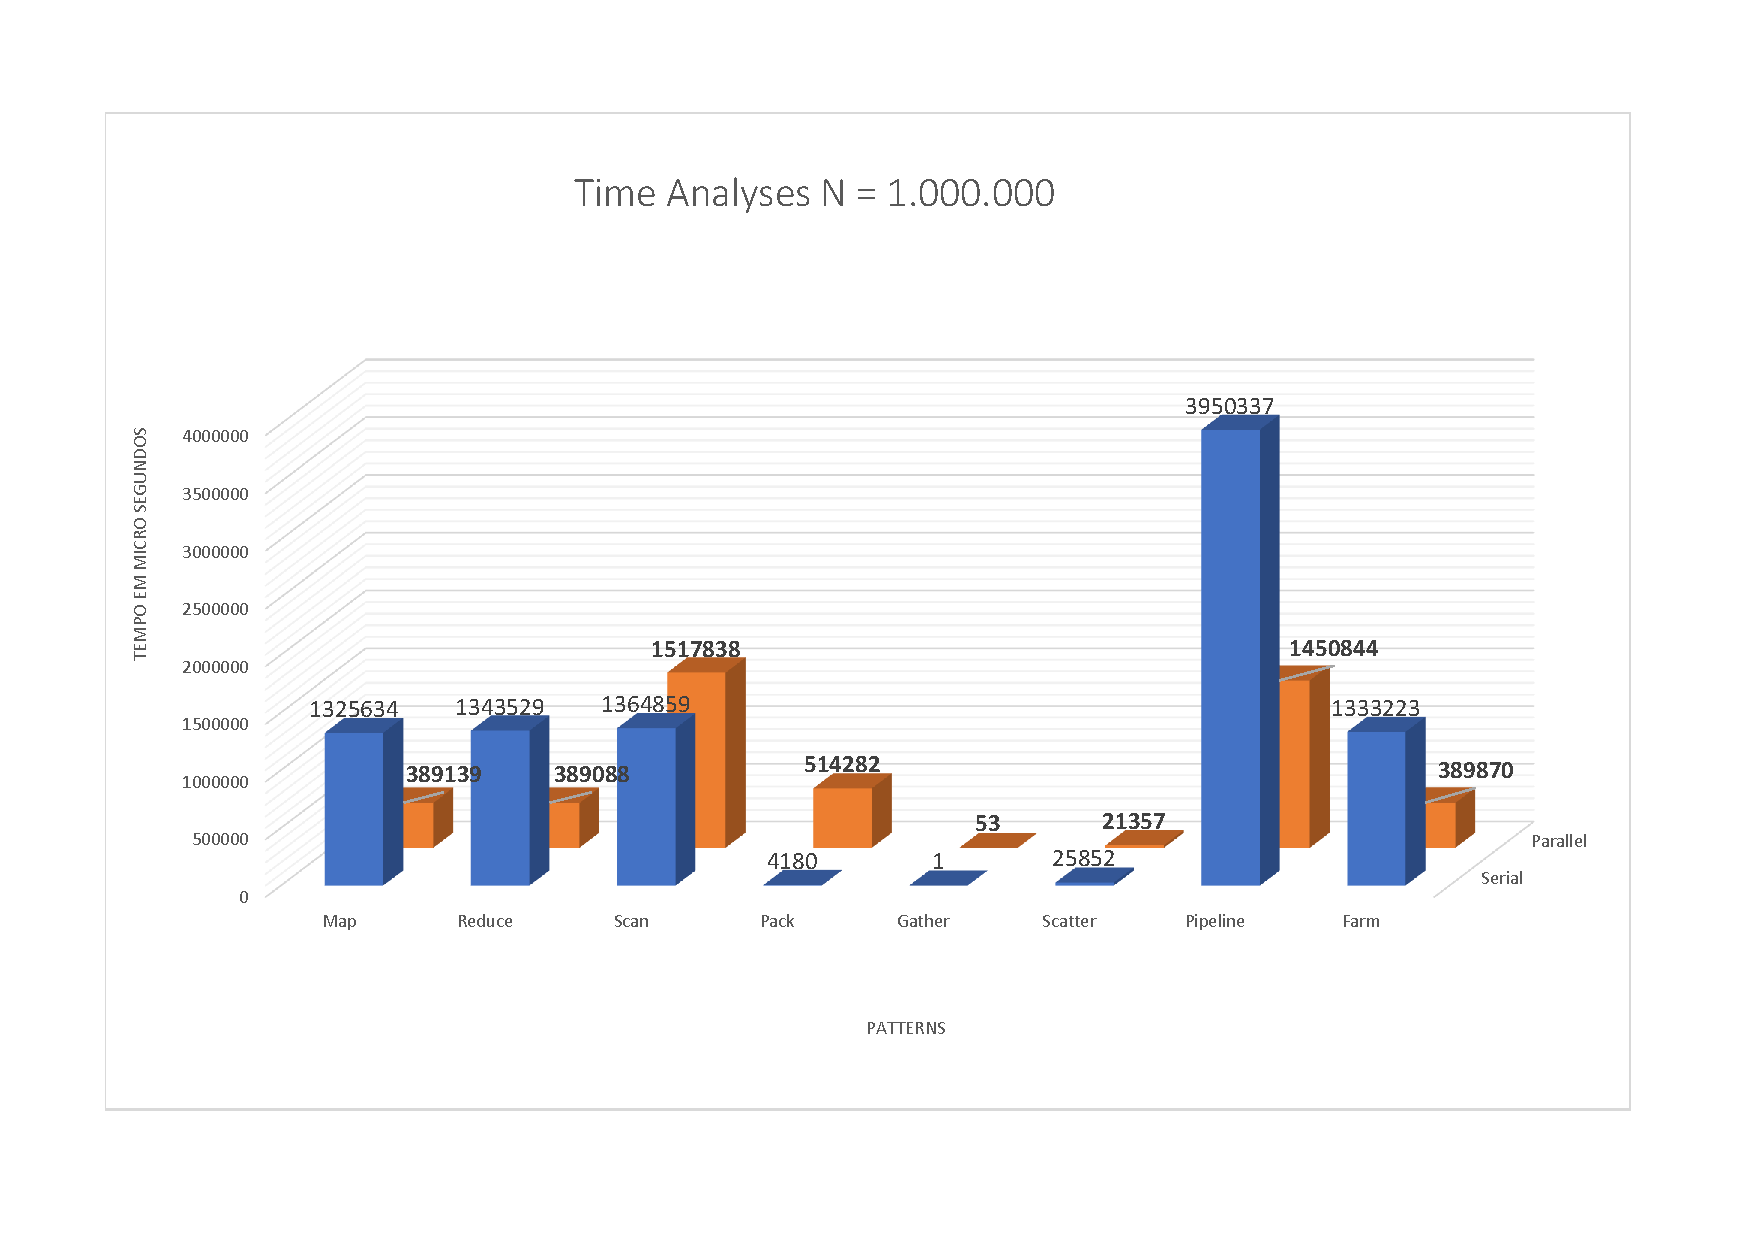
\includegraphics[height=6cm,width=9.44cm]{jpeg/n=1000000.pdf}
\caption{N=1.000.000}
\label{figura:n1000000}
\end{figure}

For N=1.000.000 represented in (Fig. 4.) we kept with almost no proportional changes between serial and parallel times but a small decreasing on parallel times in compare with serial.

\begin{figure}[H]
\hspace*{-0.24in}
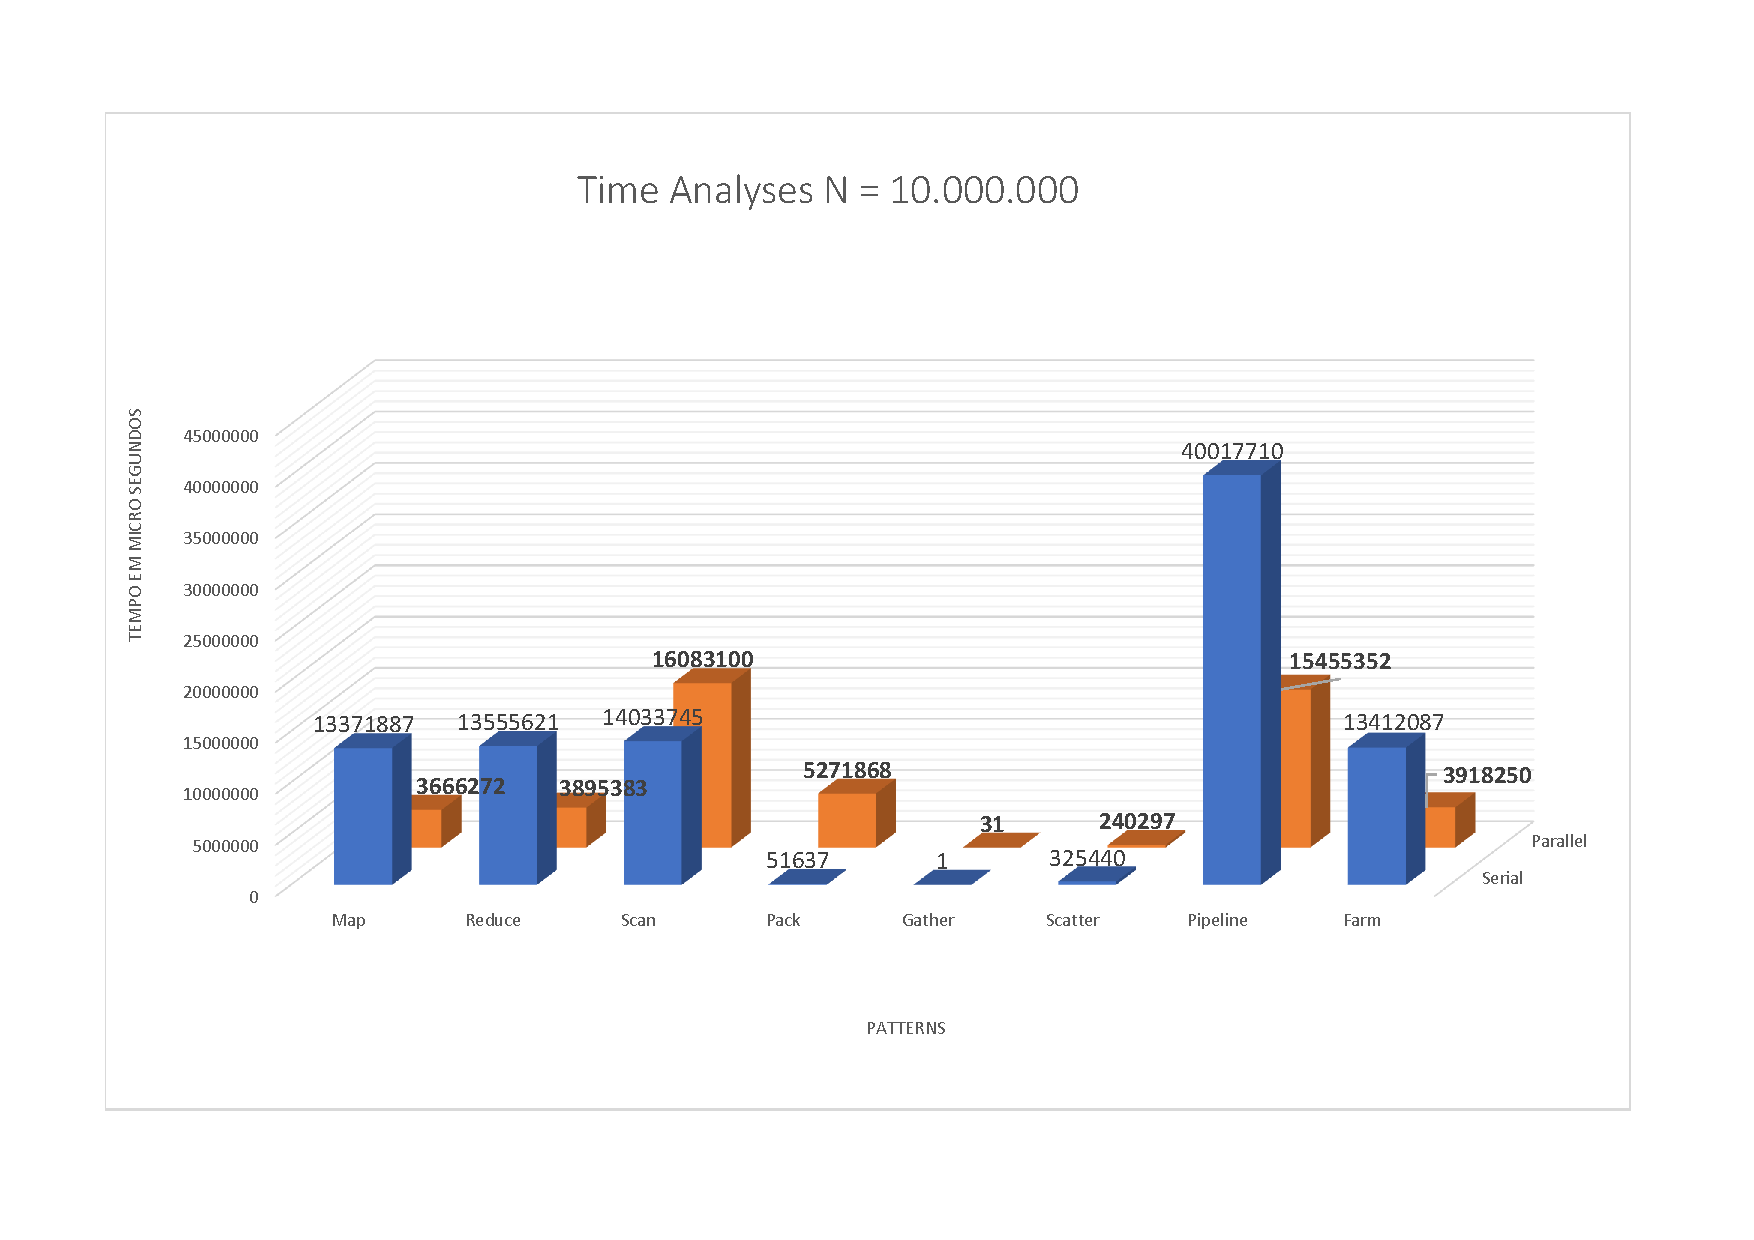
\includegraphics[height=6cm,width=9.44cm]{jpeg/n=10000000.pdf}
\caption{N=10.000.000}
\label{figura:10000000}
\end{figure}

For N=10.000.000 represented in (Fig. 5.) for our last N we can see that the pattern holds still so there's not much higher gains for now on so we can assume we've reached a bottleneck and there's no need to tens any higher value of N.


\begin{figure}[H]
\hspace*{-0.24in}
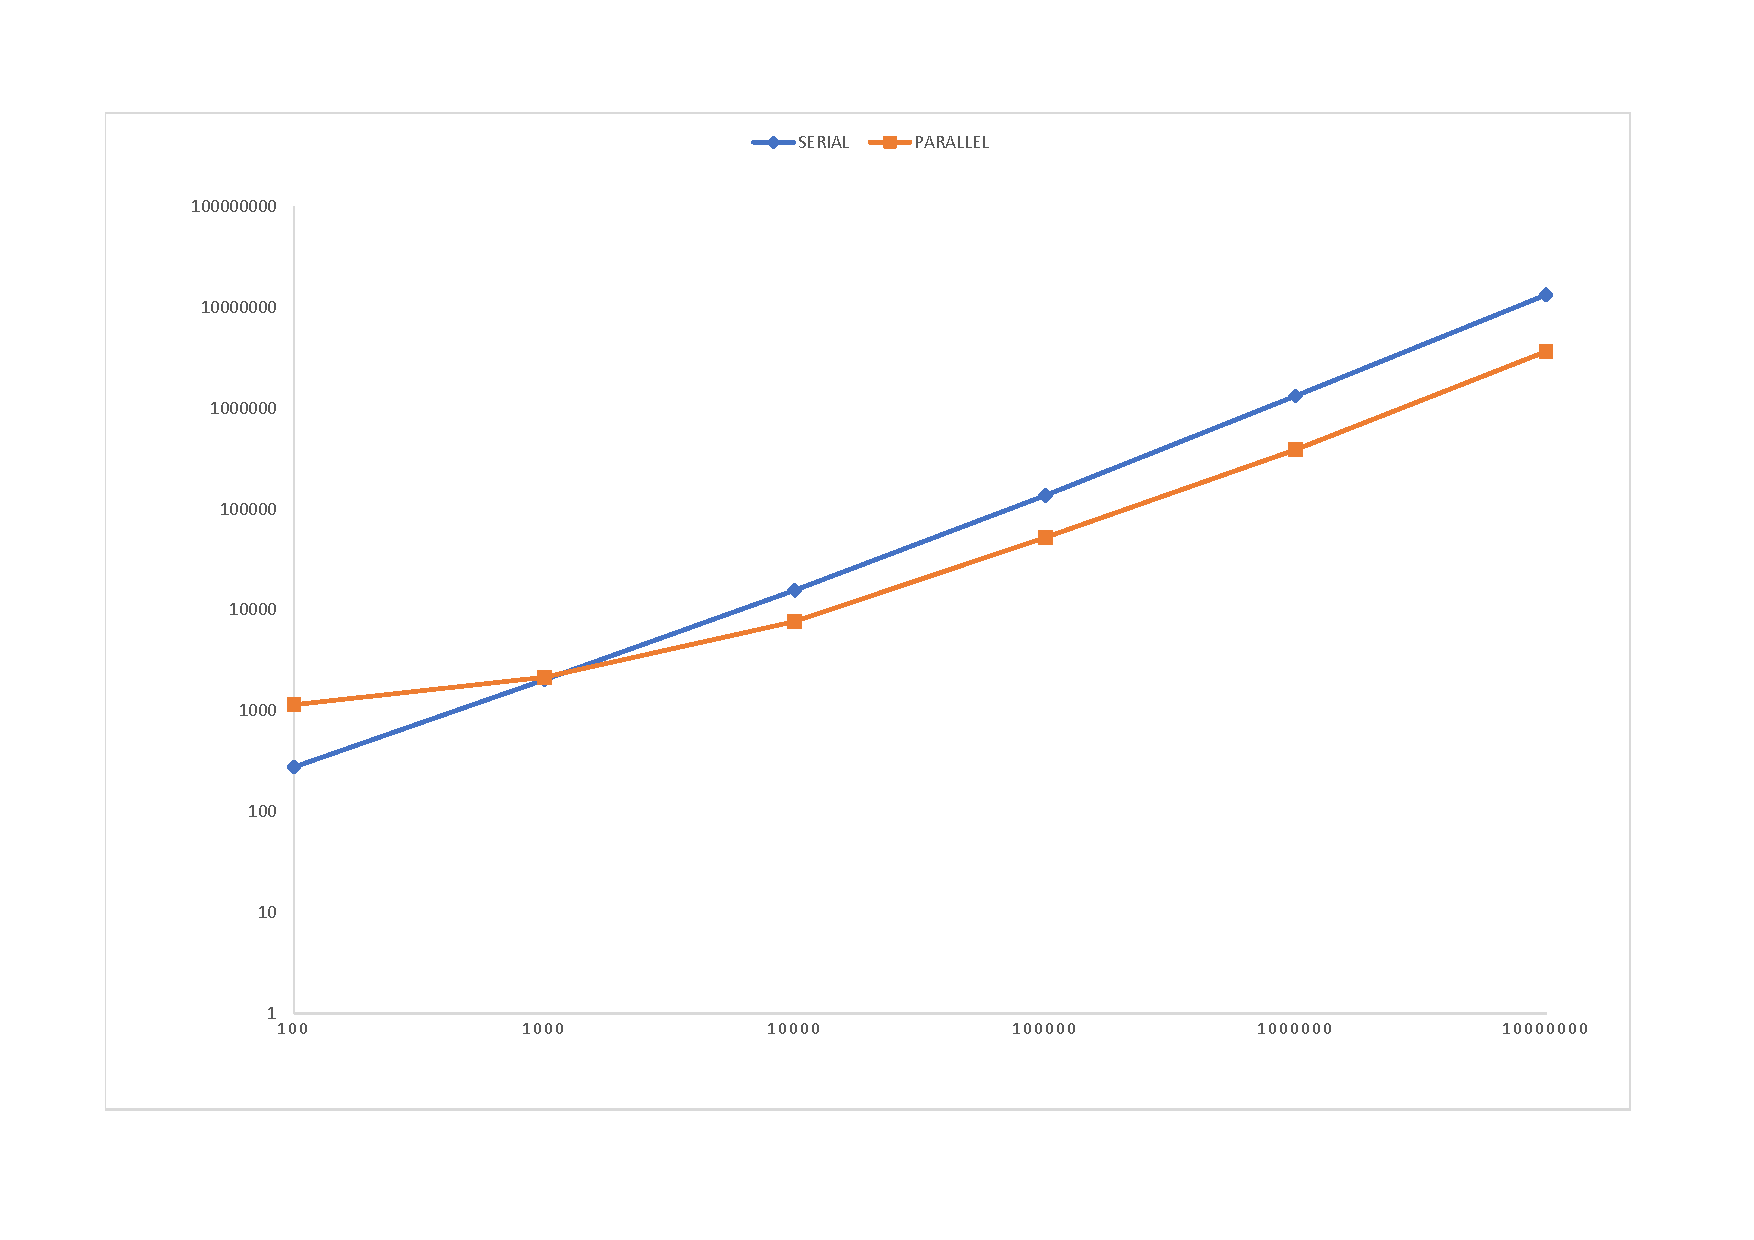
\includegraphics[height=6cm,width=9.44cm]{jpeg/map-graph.pdf}
\caption{Map Graph}
\label{figura:map}
\end{figure}

\begin{figure}[H]
\hspace*{-0.24in}
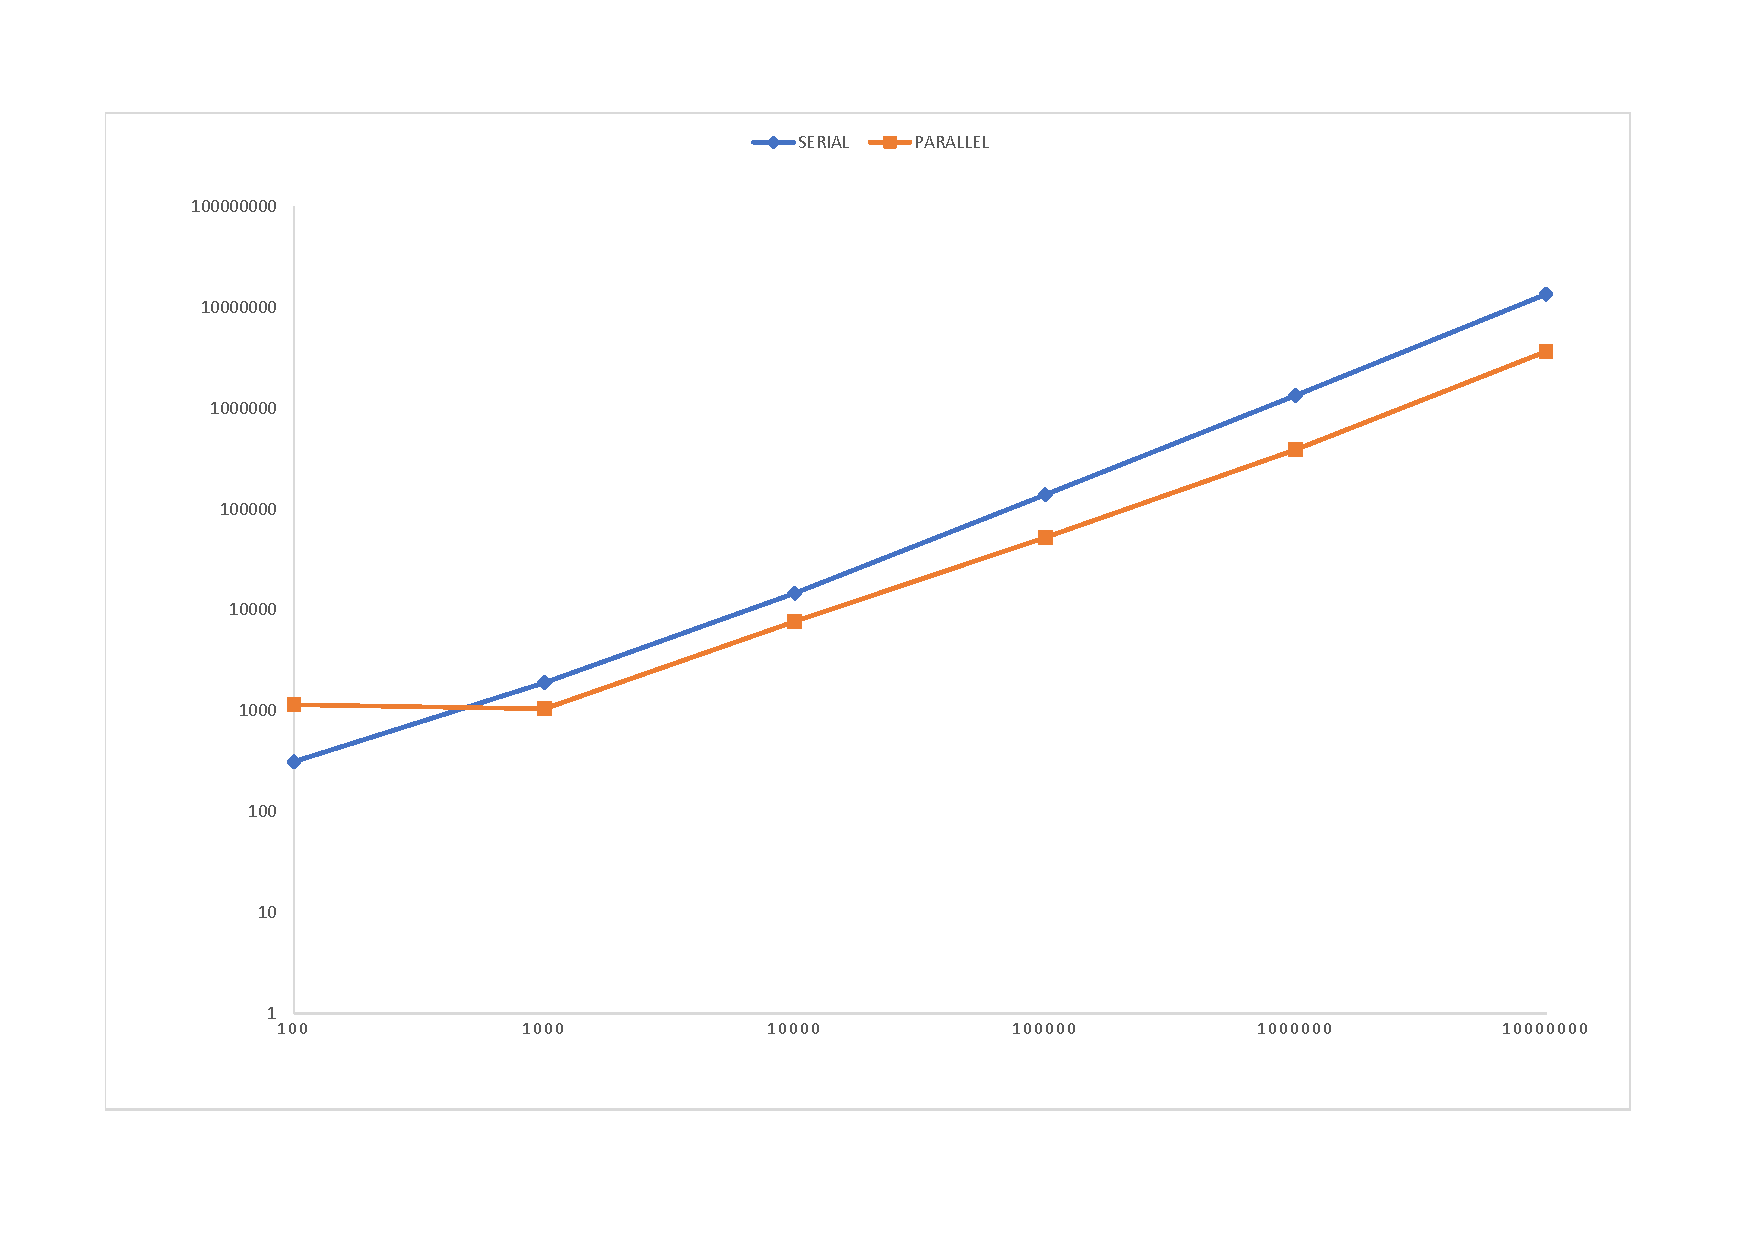
\includegraphics[height=6cm,width=9.44cm]{jpeg/reduce-graph.pdf}
\caption{Reduce Graph}
\label{figura:reduce}
\end{figure}

\begin{figure}[H]
\hspace*{-0.24in}
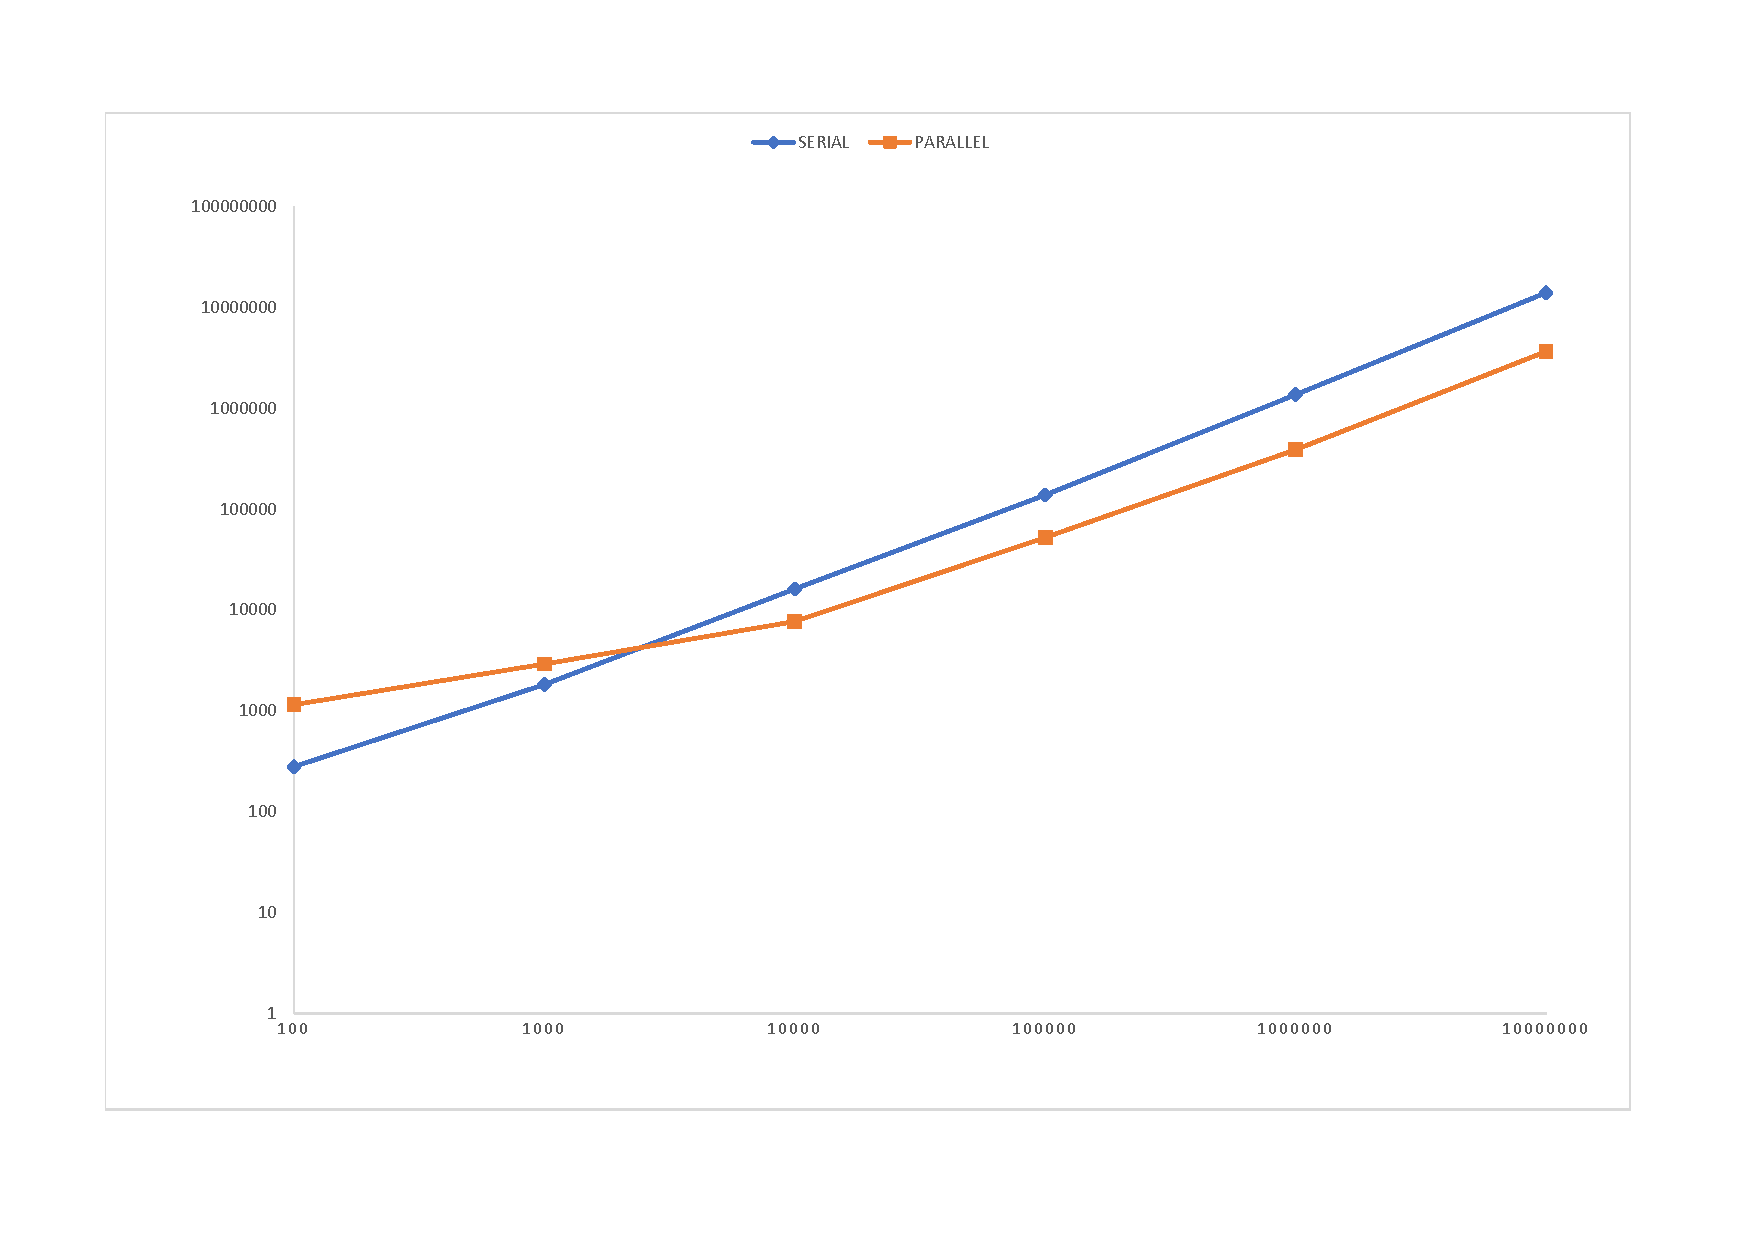
\includegraphics[height=6cm,width=9.44cm]{jpeg/scan-graph.pdf}
\caption{Scan Graph}
\label{figura:scan}
\end{figure}

\begin{figure}[H]
\hspace*{-0.24in}
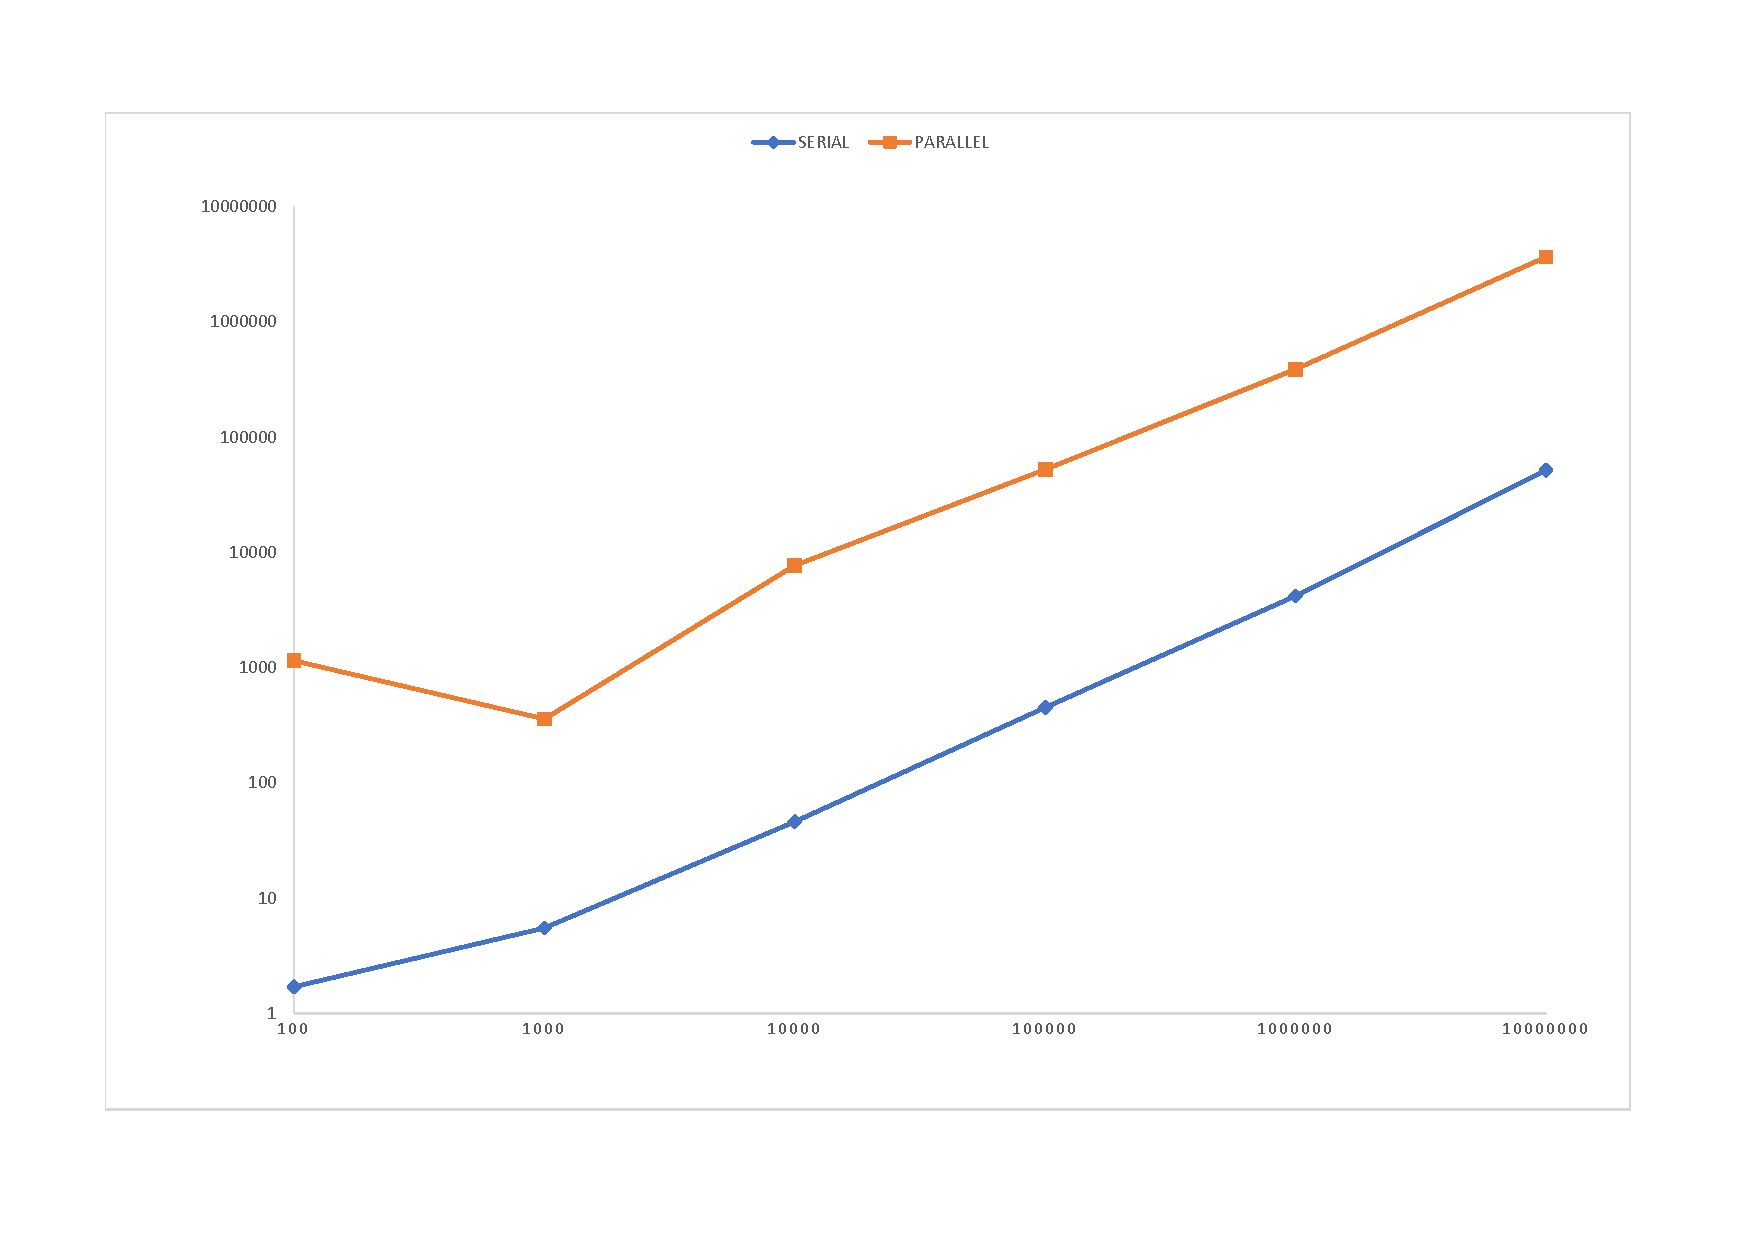
\includegraphics[height=6cm,width=9.44cm]{jpeg/pack-graph.pdf}
\caption{Pack Graph}
\label{figura:pack}
\end{figure}

\begin{figure}[H]
\hspace*{-0.24in}
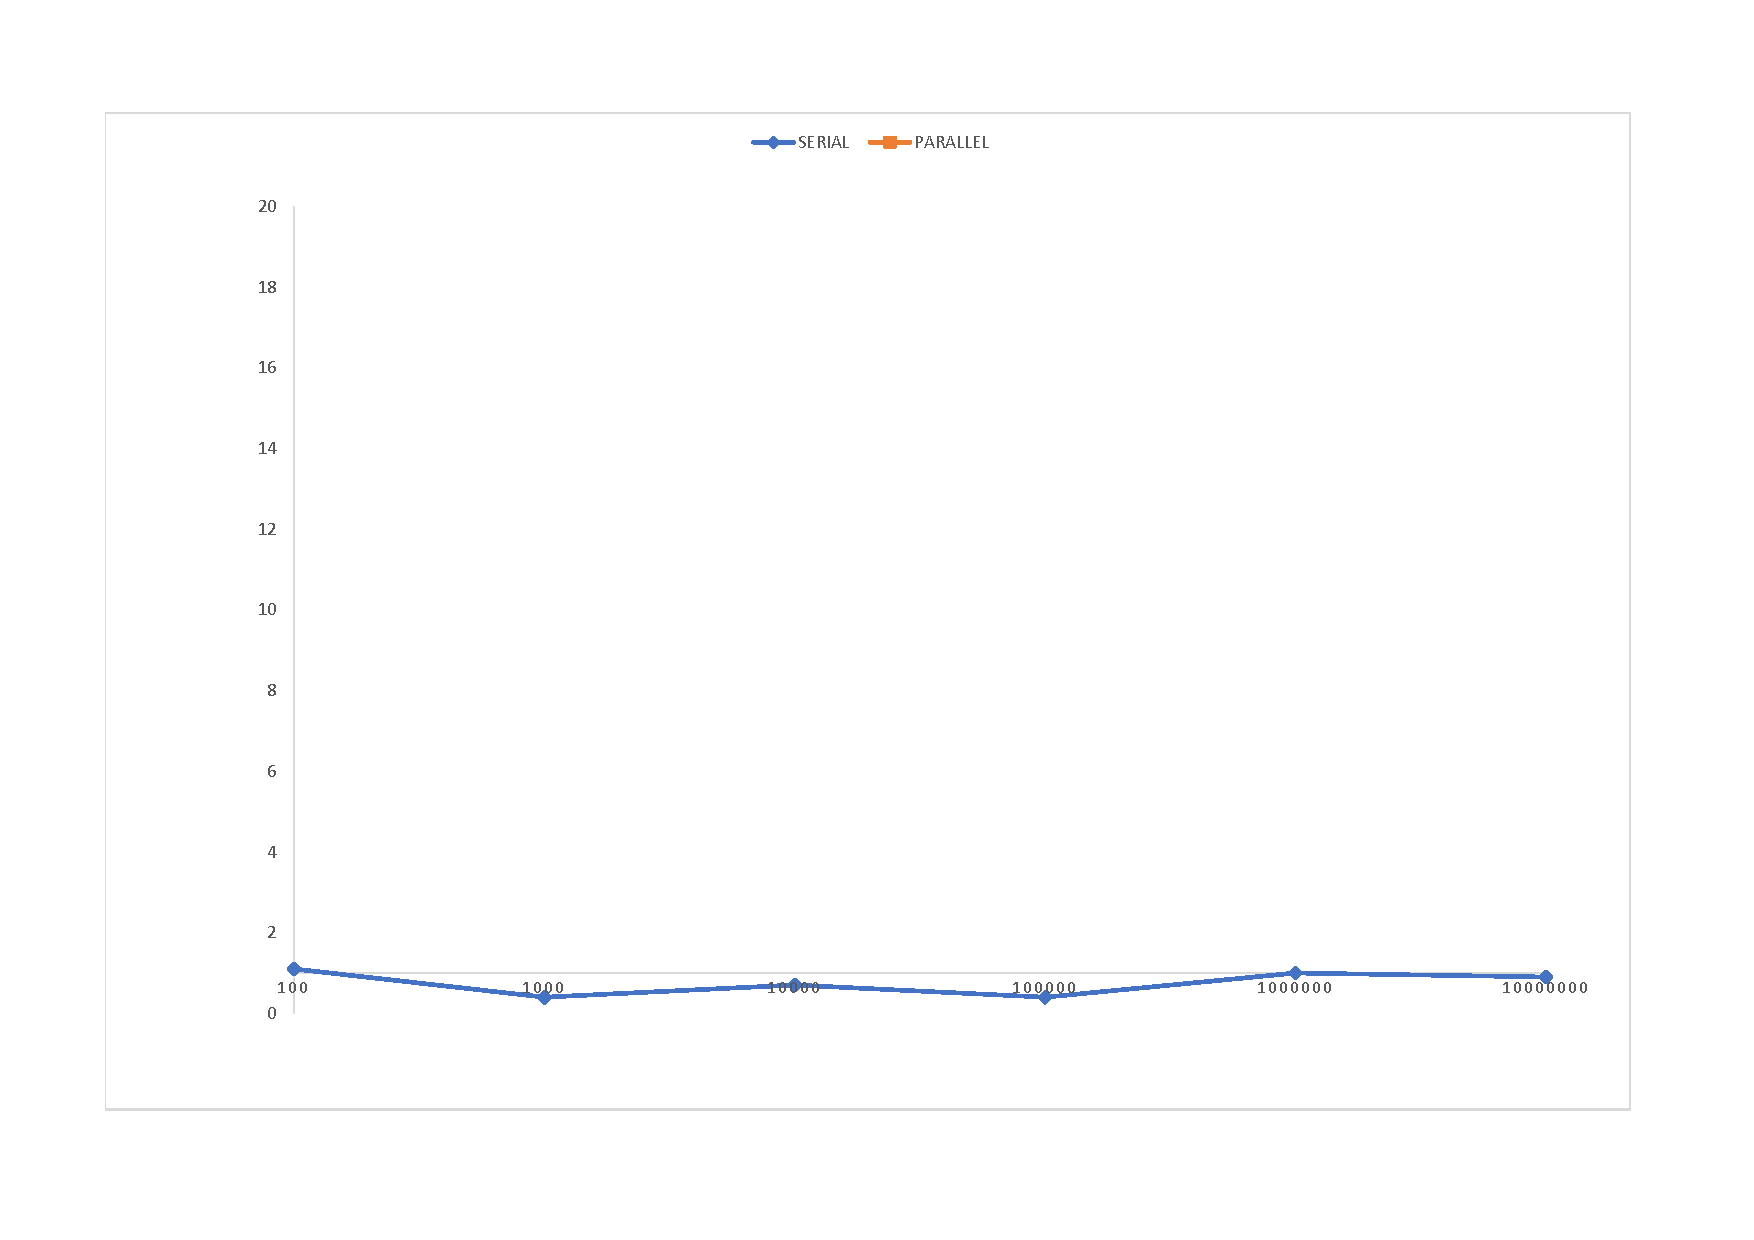
\includegraphics[height=6cm,width=9.44cm]{jpeg/gather-graph(problem).pdf}
\caption{Gather Graph}
\label{figura:gather}
\end{figure}

\begin{figure}[H]
\hspace*{-0.24in}
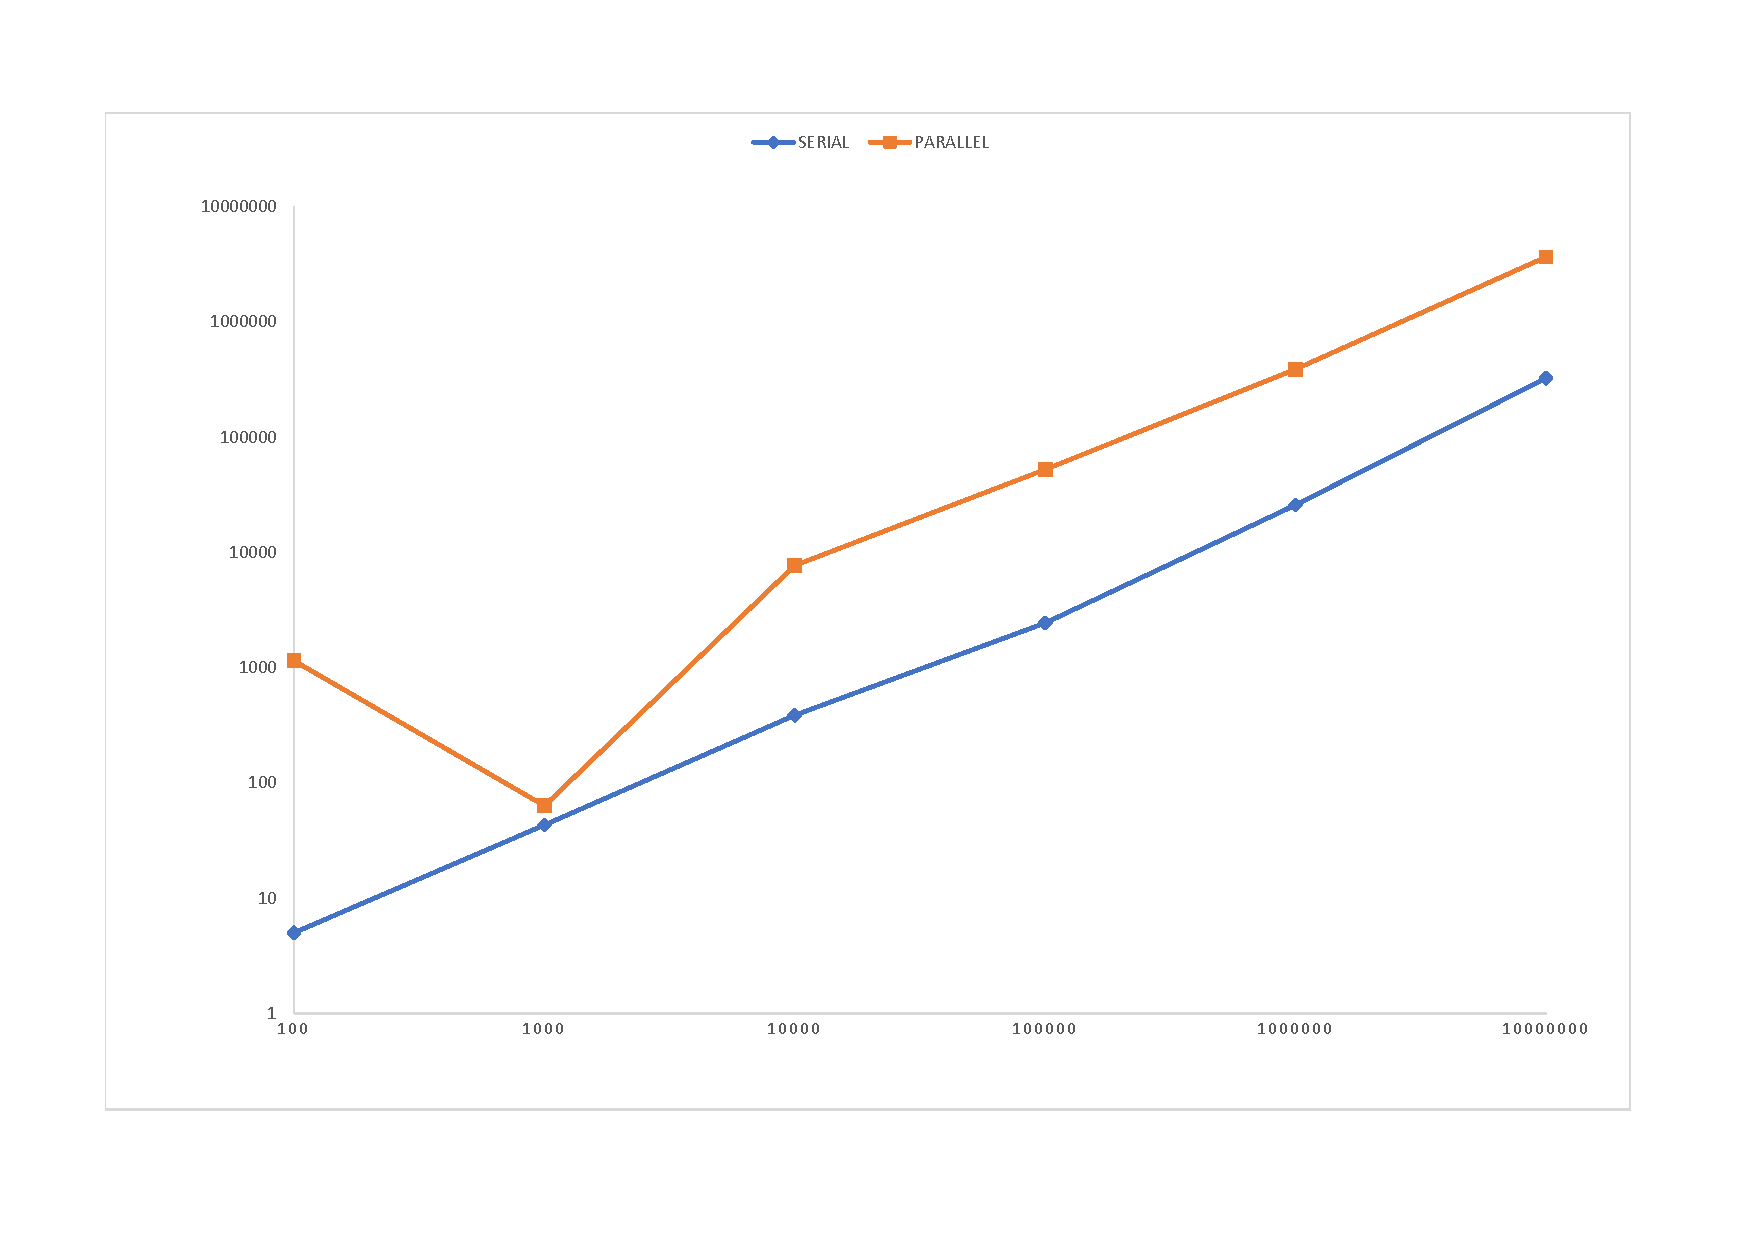
\includegraphics[height=6cm,width=9.44cm]{jpeg/scatter-graph.pdf}
\caption{Scatter Graph}
\label{figura:scatter}
\end{figure}

\begin{figure}[H]
\hspace*{-0.24in}
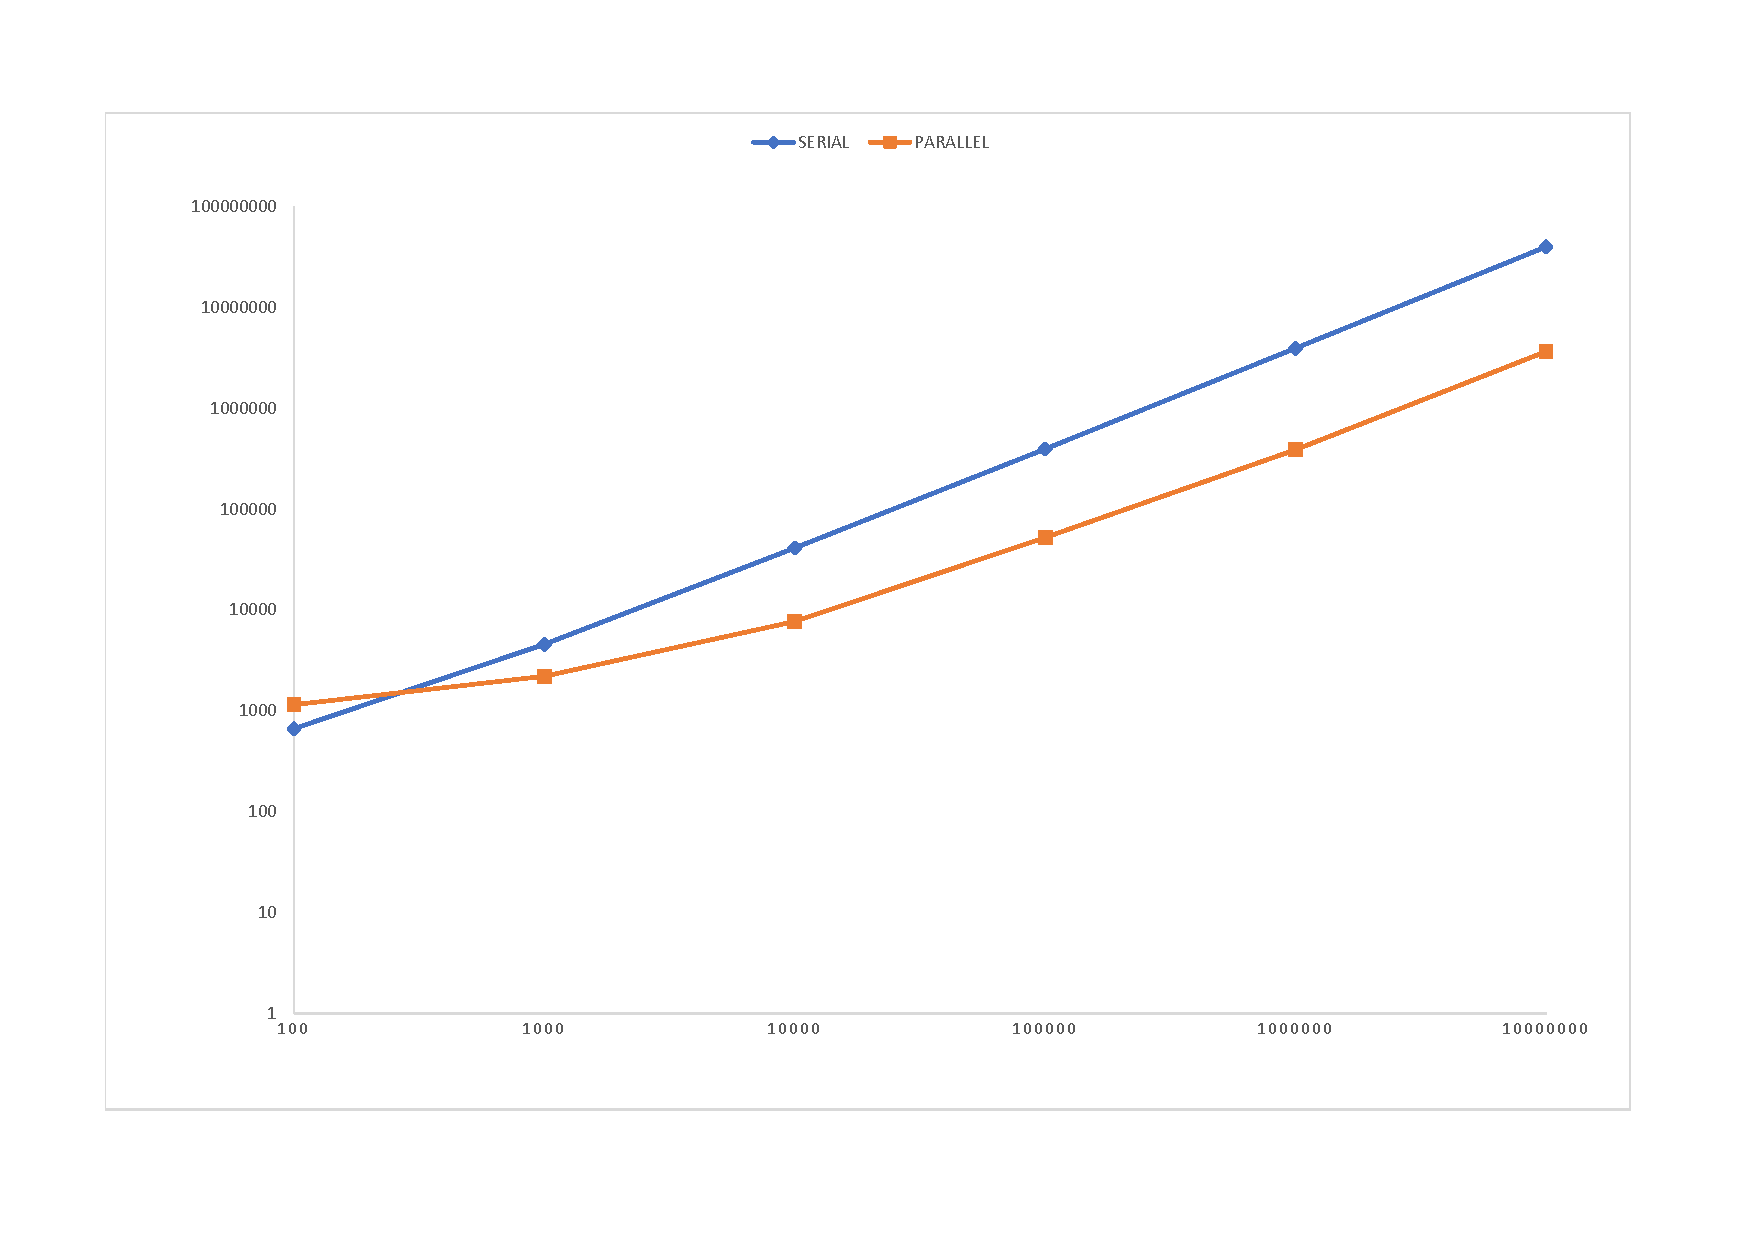
\includegraphics[height=6cm,width=9.44cm]{jpeg/pipeline-graph.pdf}
\caption{Pipeline Graph}
\label{figura:pipeline}

\end{figure}

\begin{figure}[H]
\hspace*{-0.24in}
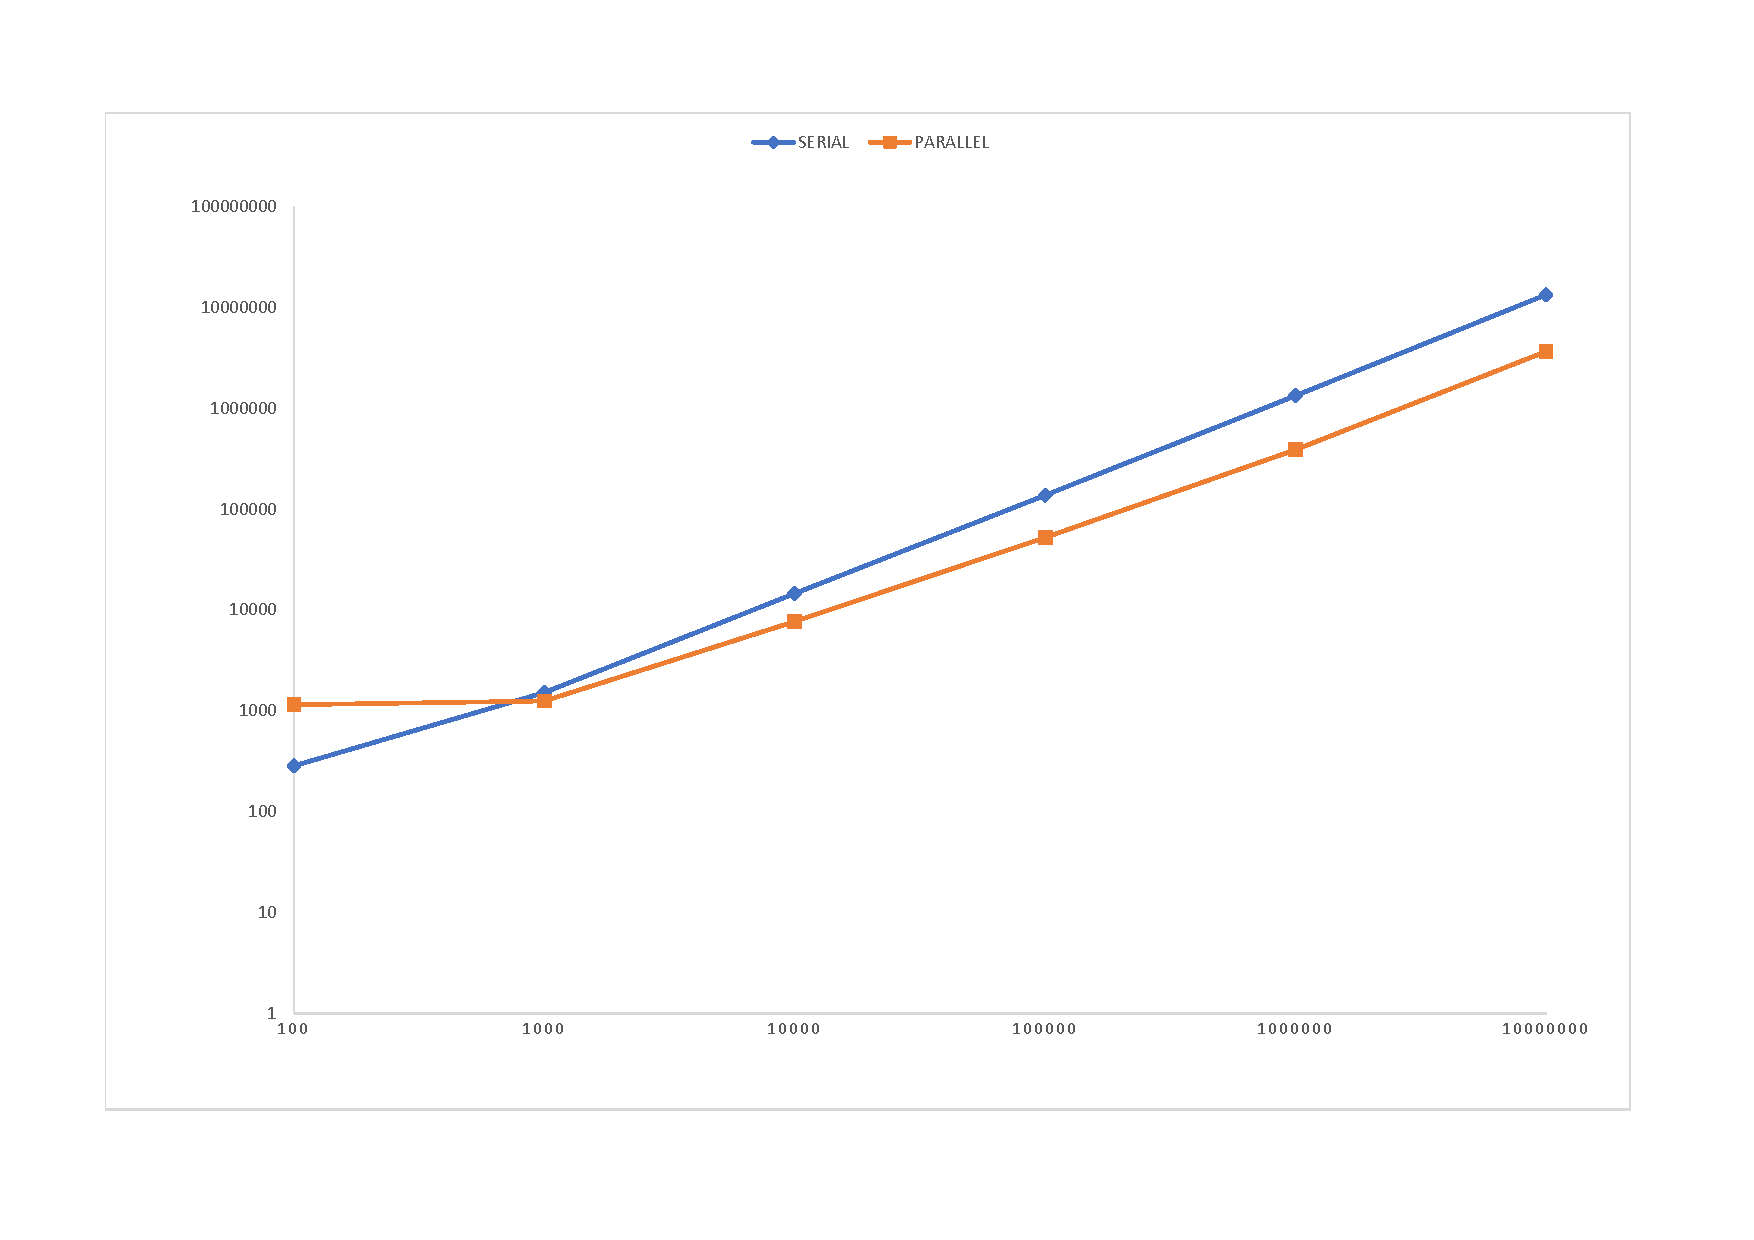
\includegraphics[height=6cm,width=9.44cm]{jpeg/farm-graph.pdf}
\caption{Farm Graph}
\label{figura:farm}
\end{figure}

The previous images, from Fig. 7. to Fig. 14. show a logarithmic representation of the relation between N (size of the problem) X axis and time Y axis. We can see that all parallel times start with higher levels in compare with serial times. 

But then, except for Pack and Scatter patterns, on all other patterns around N=1.000 serial and parallel lines cross each other and parallel times become lower than serial. Until N = 10.000.000 the evolution of the relations keeps almost linear with parallel times slightly better than serial times.

For Pack and Scatter patterns the serial is always faster than parallel, so we conclude that with the input given for the experiments,  the work performed by the workers is not big enough to overcame the scheduling overheads of parallelism.

\section{Conclusion}
This Project gave us a wider view of a common problem known in the Computing world, and how to overcome it, and acknowledge as well, that Parallel Patterns do not mean faster performance in comparison to the Serial Patterns in all circumstances.

After the implementation of the project, and extend analysis of the outcome given by our experiments, we can conclude that all patterns can be successfully parallelized. Said that, we cannot strongly state it is true for all cases and for any experiment that we may make. Each result, and improvement depends not only on the best possible solution of a pattern, but specially the variables that we are working in each environment.

Finally, we are pleased with the results that we achieved, in our point of view, we successfully overcome the difficulties of this project, and we tried to expose all the variables that we can or we encounter testing, in order to prove all advantages and disadvantages of parallelizing a program, when or why is truly worth it of using it.



\section*{Acknowledgement}

We would like to give a special thanks to the group G28,  which helped us to overcome some issues, without giving us the solution, but making us go in the right direction.

\begin{thebibliography}{1}

\bibitem{1}
Michael McCool, Arch D. Robison, James Reinders, \emph{Structured Parallel Programming Patterns for Efficient Computation}, 2012.\hskip 1em plus
  0.5em minus 0.4em\relax Morgan Kaufmann, 2012 Elsevier.
  
\bibitem{2}
Maurice Herlihy , Nir Shavit, \emph{The Art of Multiprocessor Programming}, 2008.\hskip 1em plus
  0.5em minus 0.4em\relax Morgan Kaufmann, 2008 Elsevier.
  
\bibitem{3}
Michel Raynal, \emph{Concurrent Programming: Algorithms, Principles, and Foundations}, 2013.\hskip 1em plus
  0.5em minus 0.4em\relax Springer-Verlag Berlin Heidelberg 2013.  
  
\bibitem{4}
Jo\~ao Louren\c{c}o, \emph{ Concurrent and Parallelism - Lectures, T10}, 2018.\hskip 1em plus
  0.5em minus 0.4em\relax Faculdade Ci\^encias e Tecnologias, Universidade Nova de Lisboa.  
  
\bibitem{5}
\emph{http://www.drdobbs.com}

\end{thebibliography}

\end{document}


